\documentclass[sigconf, 10pt]{acmart}

% NOTE: acmart fixes the text block to the MobiCom-mandated column geometry
% (9.25in x 3.33in, 0.33in gutter, <=55 lines/column). Do NOT load geometry,
% and do not change \baselinestretch -- either silently violates the CFP.
\usepackage[english]{babel}
\usepackage{caption}
\usepackage{color}
\usepackage{tabularx}
\usepackage{multirow}
\usepackage{graphicx}
\usepackage{xcolor} % For custom colors
\usepackage{array} % To use the 'p' column type
\usepackage{makecell} % To allow for line breaks within cells
\usepackage{booktabs} % For better table lines
\usepackage{microtype}
\usepackage{amssymb}
\usepackage{tikz}
\usepackage{pgfplots}
\pgfplotsset{compat=1.18}
\usetikzlibrary{arrows.meta,positioning,fit,calc,backgrounds,shapes.geometric,decorations.pathreplacing}
\tolerance=1500

% --- shared TikZ styles for the HALO figures (see figures/*.tex) ---
\definecolor{haloblue}{RGB}{31,90,150}
\definecolor{haloorange}{RGB}{205,110,30}
\definecolor{halogreen}{RGB}{40,125,85}
\definecolor{halogray}{RGB}{110,110,115}
\definecolor{halolight}{RGB}{232,240,248}
\definecolor{halolight2}{RGB}{252,240,226}
\tikzset{
  hbox/.style={draw=haloblue!70,fill=halolight,rounded corners=2pt,inner sep=3pt,
               align=center,font=\scriptsize},
  hbox2/.style={draw=haloorange!70,fill=halolight2,rounded corners=2pt,inner sep=3pt,
                align=center,font=\scriptsize},
  hplain/.style={align=center,font=\scriptsize,inner sep=2pt},
  harrow/.style={-{Latex[length=1.5mm,width=1.2mm]},draw=halogray,thick},
  fbok/.style={draw=haloblue!70,fill=haloblue!55,minimum size=2.9mm,inner sep=0pt,rounded corners=0.3pt},
  fbblur/.style={draw=haloblue!70,fill=haloblue!18,minimum size=2.9mm,inner sep=0pt,rounded corners=0.3pt},
  fbno/.style={draw=halogray!55,fill=halogray!10,minimum size=2.9mm,inner sep=0pt,rounded corners=0.3pt},
  hphase/.style={draw=halogray!60,dashed,rounded corners=3pt,inner sep=5pt},
}

% Tighten float spacing
\setlength{\textfloatsep}{8pt plus 2pt minus 2pt}
\setlength{\floatsep}{6pt plus 2pt minus 2pt}
\setlength{\intextsep}{6pt plus 2pt minus 2pt}
\setlength{\dbltextfloatsep}{8pt plus 2pt minus 2pt}
\setlength{\dblfloatsep}{6pt plus 2pt minus 2pt}

% Copyright
\renewcommand\footnotetextcopyrightpermission[1]{} % removes footnote with conference info
\setcopyright{none}

%\setcopyright{acmcopyright}
%\setcopyright{acmlicensed}
%\setcopyright{rightsretained}
%\setcopyright{usgov}
%\setcopyright{usgovmixed}
%\setcopyright{cagov}
%\setcopyright{cagovmixed}

\newcommand{\name}{HALO\xspace}

\def\thickhline{\noalign{\hrule height.8pt}}

\newcommand{\TODO}[1]{{\color{red}{#1}}}

% --- FORWARD-LOOKING placeholders ------------------------------------------------
% These mark space reserved for content that does not exist yet. They never refer to
% superseded work: anything inconsistent with the current design is deleted outright,
% so the manuscript states one version of the project and nothing else.
%
%   \PENDING{...}   a visible orange note: "this will be written once the run lands"
%   \PH             one orange placeholder cell inside a results table
%   \PHFIG{h}{...}  an orange box of height h reserving space for a figure
\newcommand{\PENDING}[1]{{\color{orange}\textbf{[TO BE COMPLETED]} \textit{#1}}}
\newcommand{\PH}{{\color{orange}\rule[-0.15ex]{1.6em}{0.9ex}}}
\newcommand{\PHFIG}[2]{%
  \begingroup\color{orange}%
  \fboxsep=0pt\fboxrule=0.8pt%
  \fcolorbox{orange}{orange!7}{%
    \parbox[c][#2][c]{\dimexpr\columnwidth-2\fboxrule\relax}{\centering\itshape #1}}%
  \endgroup}

\pagestyle{plain} % removes running headers
\settopmatter{printacmref=false, printccs=false, printfolios=true}
% \acmConference[SIGCOMM '23]{SIGCOMM '23: Annual conference of the ACM Special Interest Group on Data Communication}{Sep 2023}{New York City, US}

% DOI
\acmDOI{}

% ISBN
\acmISBN{}

%Conference
%\acmConference[Submitted for review to SIGCOMM]{}
%\acmYear{2018}
%\copyrightyear{}

%% {} with no args suppresses printing of the price
% \acmPrice{}


\begin{document}

\title{HALO: A Heterogeneity-Aware, Language-Conditioned IMU Foundation Model for Label-Efficient Human Activity Recognition}

% Compared with image and text; sensing is a lot more heterogeneous, sample rate, sensor charateristics, and modalities; when it comes to training large models benefit on large scale data, it proposes challenges


% \title{MMBind: Multimodal Learning for IoT through Binding Distributed and Incomplete Data
% }
% MMBind: Multimodal Learning on Distributed Incomplete IoT Data via Binding with Common Modality

% author list: Xiaomin, Jason (co-first), Tommy, Yihan, xxx (professors and collaborators)


% Learning algorithms and models for perception, understanding, and adaptation

%\titlenote{Produces the permission block, and copyright information}
%\subtitle{Extended Abstract}
% Paper #N, 12 pages body, 14 pages total
% \author{Paper \#239, 12 pages body, 17 pages total}
% \author{Firstname Lastname}
% \authornote{Note}
% \orcid{1234-5678-9012}
% \affiliation{%
%   \institution{Affiliation}
%   \streetaddress{Address}
%   \city{City} 
%   \state{State} 
%   \postcode{Zipcode}
% }
% \email{email@domain.com}

% The default list of authors is too long for headers}
% \renewcommand{\shortauthors}{xxx}
% yet no single model can accept diverse IMU configurations---varying sampling rates, channel counts, and sensor placements---and recognize activities across unseen devices and label vocabularies without per-dataset adaptation.
\begin{abstract}
Human activity recognition has no foundation model a developer can simply pick up: one pretrained
model that reads whatever sensors a device exposes, recognises the application's own activity
names, and needs only as much labelled target data as the deployment can afford. The field has
pursued this through scale, but inertial signals admit no closed grammar the way language
does---a change of mounting, placement, sampling rate, or on-device filtering puts a recording
outside any corpus---so compatibility with an unseen configuration must be built in as inductive
bias rather than accumulated as coverage. A second obstacle is that the standard remedy for open
label sets, projecting sensor features into a sentence-embedding space, presumes that sensor
similarity tracks linguistic similarity. It does not, and it fails in both directions:
\emph{drinking coffee} and \emph{drinking water} are one wrist motion but distant strings, while
\emph{sitting} and \emph{sitting down}---a posture and a transition---are nearly identical ones.
We present HALO (\textbf{H}eterogeneity-\textbf{A}ware \textbf{L}anguage-conditioned
\textbf{O}pen-set model)\footnote{Source code and pretrained models will be released upon
acceptance.}, which answers each obstacle with a design choice. A tokenizer with
\emph{calibrated} inductive bias groups co-located axes into sensors and reads each on a fixed
physical-frequency axis, so the representation is rate-invariant and anti-aliased \emph{by
construction}, with per-token masks declaring what a given rate and window could not observe;
sensor identity enters as language attached to the sensor, leaving channel count and ordering
free while staying too coarse to fingerprint a corpus. An \emph{evidence engine} then declines to
reconcile the two geometries at all, retrieving encoded exemplars from a memory by \emph{sensor}
similarity and accumulating evidence for whichever labels the deployment declares at run time.
Pretraining uses no activity labels. The result is one \emph{label-efficiency curve} rather than
a zero-shot-versus-fine-tuning dichotomy: a single frozen model spans no target data, a handful
of demonstrations appended to memory with no gradient update, and full supervision. We train on
12 public datasets spanning 20 sensor streams and evaluate on 7 held-out datasets under a
leakage-free, subject-disjoint protocol scored against each dataset's own label strings.
\end{abstract}


\maketitle

\section{Introduction}

A physiotherapist may ask a patient recovering from knee surgery to perform six exercises at home.
The patient already owns a phone and a watch, but the exercise set was selected for that patient and
may not appear in a public dataset. Collecting enough annotated examples to train a new model for
every device and placement is rarely practical. Most inertial human activity recognition (HAR)
systems assume the opposite setting: they fix the sensor layout and activity set, collect an
annotated dataset, and fit a classifier for that combination.

We study a setting with three requirements. First, the activity set is \emph{open}: an application
supplies its candidate names at inference, including names absent from pretraining. Second, the
input is \emph{heterogeneous}: devices differ in placement, modality, channel availability,
sampling regime, gravity convention, and filtering. Third, a deployment may provide zero, one, or a
few labeled examples of each candidate. These requirements interact. A stored wrist example may be
useful for recognizing an arm exercise from another wrist device, but it should not decide an arm
gesture observed only by a pocket phone, however close their embeddings happen to be.

Two limitations motivate HALO.

\textbf{(L1) Acquisition configuration changes what evidence is observable.}
Rotation, placement, sampling, firmware filtering, and sensor availability jointly change the
recorded signal. A larger corpus improves coverage but cannot enumerate their continuous
combinations. Nor does resampling make two instruments equivalent: interpolation cannot recover
frequencies that the acquisition clock or device filter removed. We therefore expose selected
configuration facts to both the representation and the retrieval rule.

\textbf{(L2) A geometric neighbor is not automatically admissible evidence.}
Open-label methods often align sensor features with activity-name embeddings and classify by text
similarity~\cite{clip,lanhar,goat}. Yet language encodes objects and goals that an IMU may not
observe, while small wording changes may distinguish a posture from a transition. We consequently
compare recordings in sensor space, but condition the right to vote on whether the query and stored
sensor configurations can observe the candidate concept. Section~\ref{sec:geometry} gives concrete
counterexamples without treating author-assigned motion relations as quantitative ground truth.

\textbf{HALO.} HALO has a label-free representation stage and an evidence stage. The tokenizer
defines frequency bands in physical hertz on the stored grid, preserves signed low-frequency
acceleration, and marks bands unavailable under the acquisition rate or unresolved by the patch
duration. It folds the axes of each accelerometer or gyroscope into a sensor token with an explicit
axis-validity mask. The token also receives a frozen text description and activity-invariant
acquisition statistics. Phase A learns from masked contextual prediction, reconstruction of hidden
sensor descriptions, and consistency across physical augmentations.

At inference, the encoder is frozen. A versioned memory stores one row per patch and sensor, with
label and provenance. The evidence path applies hard modality/gravity compatibility, a learned
low-rank admissibility gate, cosine ranking within the surviving rows, voting, and closed-form
sensor fusion. A labeled demonstration is appended to memory and bound directly to the application's
candidate; it does not trigger a gradient update. Candidate names enter at run time rather than
through a fixed classifier head.

This paper makes four contributions. First, it specifies a sensor-granular tokenizer whose frequency
coordinates and missing-information masks retain acquisition meaning. Second, it formulates
retrieval admissibility as a separate, observable question from feature similarity. Third, it
defines a leakage-aware enrollment protocol with support-removal, support-label-shuffling,
ungated-retrieval, prototype, and ridge controls. Fourth, it reports the current negative development
result: the fitted gate uses the support but does not beat simpler controls. This bounds the present
claim and identifies what must improve before the sealed test roster is evaluated.


\section{Related Work}
\label{sec:related}

HALO sits at the intersection of four literatures, and in each of them some part of what we do
already exists. We name the closest work in each and state what is left.

\textbf{Cross-dataset and foundation models for IMU sensing.}
Deep HAR has moved from single-dataset CNN--LSTM models~\cite{deepconvlstm} through methods that
attack one axis of heterogeneity at a time---contrastive fusion for small-data multimodal
HAR~\cite{cosmo}, physics-informed augmentation for cross-user and cross-device
transfer~\cite{unihar}, federated modelling of inter-user structure~\cite{clusterfl}---to
self-supervised encoders intended to transfer: LiMU-BERT~\cite{limubert} pretrains by span-masked
reconstruction at $20$\,Hz, CrossHAR~\cite{crosshar} combines masked reconstruction with
contrastive learning, and ssl-wearables~\cite{sslwearables} scales multi-task self-supervision to
roughly $700$k person-days of wrist accelerometry. A second wave targets foundation-scale
wearable modelling: LSM~\cite{lsm1} establishes the label-efficiency argument (up to $8\times$
fewer labelled examples), LSM-2~\cite{lsm2} learns directly from incomplete recordings,
RelCon~\cite{relcon} learns a motion-similarity metric over $\sim\!10^9$ windows, and
SensorLM~\cite{sensorlm} pairs sensor data with hierarchical captions and reports zero-shot,
few-shot, and cross-modal retrieval together. General time-series models~\cite{moment,patchtst}
and tabular ones~\cite{mitra} trade domain-specific bias for breadth. A recent survey maps this
space~\cite{harfmsurvey}, and Inertia-1~\cite{inertia1} runs a controlled lifecycle study over
modality, placement, rate, and window length. \emph{What is left:} all of these treat sampling
rate as a preprocessing decision to be normalised away. Our argument is that this is where the
information loss happens, and Section~\ref{sec:bias_experiments} measures it rather than
asserting it.

\textbf{Sampling-rate and resolution invariance.}
This is the literature closest to our L1 mechanism, and it is not in HAR. Rate-invariant
autoencoding~\cite{rateinvae} learns representations quotiented by temporal warping;
FlowState~\cite{flowstate} builds a sampling-rate-\emph{equivariant} forecasting model on a
state-space encoder with a functional-basis decoder; universal spectral
tokenization~\cite{spectraltok} ingests native, irregular wavelength grids without resampling and
explicitly proposes the same idea for multiresolution time series. Within IMU sensing,
MoPFormer~\cite{mopformer} tokenizes into learned motion primitives to make datasets comparable,
but resamples every dataset to $100$\,Hz before quantising, so its codebook is defined over a
fixed-rate grid. \emph{What is left:} FlowState conditions on the rate---it is equivariant,
adapting its computation---whereas HALO's features are \emph{anchored} to physical Hz, so a band
denotes the same physical frequency for every device and no conditioning is required to compare
across them; and the astronomical setting of~\cite{spectraltok} has no gravity, no Nyquist
guard tied to a wearable's firmware, and no anti-aliasing consequence to demonstrate. To our
knowledge no prior HAR system claims rate-invariance by construction, and none measures what
resampling costs on held-out data---which is the experiment we run, and which we regard as the
load-bearing evidence for L1 rather than the mechanism itself.

\textbf{Language as an interface to sensors.}
Two distinct uses of language must be separated. On the \emph{output} side, aligning a modality
to sentence embeddings for open-vocabulary recognition descends from
DeViSE~\cite{devise}, ConSE~\cite{conse}, and CLIP~\cite{clip}; ImageBind~\cite{imagebind} extends
it to IMU among other modalities, and LanHAR~\cite{lanhar} and LLaSA~\cite{llasa} bring it to
HAR. On the \emph{input} side---describing the sensor rather than the activity---the lane is
crowded and recently so. GOAT~\cite{goat} supervises with natural language over both activity
labels and device on-body positions. ZeroHAR~\cite{zerohar} conditions on textual sensor
context---sensor type, Cartesian axis, body position---and aligns the motion latent to it before
aligning to activity text. CHARM and its successor~\cite{charm,sensorsvoice} feed channel-level
textual descriptions into a channel-order-equivariant transformer, and their ablation finds that
conditioning on channel identity via text is one of the largest performance drivers.
SensorLLM~\cite{sensorllm} generates per-channel descriptions to teach an LLM the sensor layout;
oneHAR~\cite{onehar} handles variable combinations of sensor positions with LLM assistance;
UniMTS~\cite{unimts} takes the complementary route of encoding placement structurally as a joint
graph with rotation-invariant augmentation. \emph{What is left, honestly:} ``sensor identity as
natural language'' is not ours to claim. Our differences are specific and narrower than the
general idea. First, granularity: ZeroHAR conditions on a fixed, closed set of categorical
attributes, whereas ours is free text and therefore composes to descriptions never seen; the
channel-description line~\cite{charm,sensorsvoice,sensorllm} is free text but attaches it
per-channel, which is exactly the configuration whose corpus-identifiability we argue against and
test in Table~\ref{tab:identity_probe}. Second, what the conditioning feeds: in all of the above
it feeds a parametric head, whereas ours feeds a non-parametric memory. Third, invariance versus
conditioning: UniMTS's rotation invariance discards orientation, and with it gravity and posture,
which conditioning preserves.

\textbf{Retrieval, memory, and few-shot recognition.}
Deciding by comparison to stored examples is old in this field and new in its current form. The
ubicomp lineage recognises gestures by template: uWave~\cite{uwave} needs a single example per
gesture and matches by dynamic time warping; Junker et al.~\cite{junker} preselect candidate
segments by similarity search before classifying, which is structurally the retrieve-then-decide
shape we use; WarpingLCSS~\cite{warpinglcss} does robust online template spotting from
crowdsourced annotations. The modern lineage is episodic and parametric---matching
networks~\cite{matchingnet}, prototypical networks~\cite{protonet}---and, in language and vision,
non-parametric memory attached to a frozen model~\cite{knnlm,rag,retro,knnvision,reco}.
Memory-modular classification~\cite{memorymodular} states our Phase-B property as its
contribution: generalise to new classes by replacing memory contents, without retraining. In
sensing specifically, RAG-HAR~\cite{raghar} performs training-free retrieval over signal
descriptors and lets an LLM decide, recognising unseen activities; ZARA~\cite{zara} retrieves
multi-sensor evidence into an LLM agent, under the same ``evidence-grounded'' name we use for a
different mechanism; and in-context time-series classifiers~\cite{timee,ticfm} take a labelled
support set and a query in one forward pass with no gradient step, collapsing zero-shot and
few-shot into a single inference mode. \emph{What is left:} not ``we retrieve.'' The specific
claim is that retrieval is performed in a space where similarity is \emph{sensor} similarity
between encoded exemplar \emph{patches}, produced by an encoder that was conditioned on
acquisition configuration---which is what lets a wrist query at an unusual rate retrieve
comparable evidence, and which descriptor-space~\cite{raghar}, LLM-agent~\cite{zara}, and
CLIP-space~\cite{sensorlm} retrieval cannot do. To that we add calibrated
rejection~\cite{selectiveclass,edl}, which none of the retrieval-based HAR systems above
provide. Section~\ref{sec:label_efficiency} reports the control that decides whether this
distinction is real: the same memory mechanism on a competitor's frozen encoder.

\textbf{Self-supervised objectives.}
Phase~A composes established pieces: contrastive~\cite{simclr,infonce} and supervised
contrastive~\cite{supcon} learning as controls; non-contrastive objectives that avoid declaring
in-batch negatives~\cite{vicreg,barlowtwins}; masked modelling from language and
vision~\cite{bert,mae}; and latent-target prediction against a momentum
teacher~\cite{byol,data2vec,ijepa}. Our time--frequency term is inspired by TF-C~\cite{tfc} but
is not faithful to it, and we say so where it is described. The contribution here is not a new
objective but the choice to remove activity labels from all of them, and the cross-placement
positives that a corpus with verified simultaneous multi-device recordings makes available.

\subsection{The Combination, and Why It Is Not a List}
\label{sec:combination}

Table~\ref{tab:coverage} summarises which axes each of the closest systems explicitly addresses.
No prior system addresses all of them, which is true but is also the least interesting thing to
say about it: ``we combine more components'' is not a contribution, and a reviewer is right to
be unmoved by a filled-in row. Variable channel counts have known solutions; variable sampling
rates have known solutions; language as a bridge to an open label vocabulary has known
solutions. We claim none of those as novel.

We make a different kind of claim: that physical-Hz \emph{anchoring} is what makes a single,
flat, cross-device memory well-posed in the first place---an \emph{enabling} result rather than
an assembly. A non-parametric memory shared across deployments requires that a query encoded on
one device and an exemplar encoded on another be comparable \emph{as vectors}, with no
per-configuration index and no conditioning step to reconcile them. Resampling does not provide
this (it discards content the two devices do not share), and rate-equivariance does not provide
it either (it relates the two by a learned transformation rather than making them the same
quantity). This is why the existing retrieval-based sensing systems retrieve somewhere
else---in hand-designed descriptor space~\cite{raghar}, through an LLM
agent~\cite{zara}, or in CLIP space~\cite{sensorlm}---and why none of them needs the property
we are claiming. Section~\ref{sec:bias_experiments} tests it directly, using recordings in
which two devices captured the same person performing the same activity at the same instant, so
that configuration is the only variable (Table~\ref{tab:crossconfig}).

Once that claim is in view, the remaining choices stop looking like options. They are
\emph{mutually entailed}---each one is what makes another valid---so the set is a consequence of
L1 and L2 rather than a collection of independently attractive features. And because ``it is
just a combination'' is an empirical objection, we answer it empirically as well: the
conventional assembly of the same ingredients---resample to a common rate, attach free text per
channel, put retrieval on top---is run as a rival arm in
Table~\ref{tab:tokenizer_ablation}, not merely argued against.

\begin{table}[t]
  \centering
  \resizebox{\columnwidth}{!}{
  \footnotesize
  \setlength{\tabcolsep}{4pt}
  \begin{tabular}{l ccccc}
    \toprule
    & \multicolumn{2}{c}{acquisition} & orient./ & label &$k$-curve \\
    \cmidrule(lr){2-3}
    System & rate & placement & gravity & interface & (no grad.) \\
    \midrule
    LiMU-BERT~\cite{limubert}, CrossHAR~\cite{crosshar} &        &        &        &        &  \\
    harnet~\cite{sslwearables}, LSM~\cite{lsm1,lsm2}    &        &        &        &        & \checkmark \\
    NormWear~\cite{normwear}                            &        & $\circ$ &    & \checkmark &  \\
    UniMTS~\cite{unimts}                                &        & \checkmark & $\circ$ & \checkmark &  \\
    ZeroHAR~\cite{zerohar}                              &        & $\circ$ &        & \checkmark &  \\
    GOAT~\cite{goat}, oneHAR~\cite{onehar}              &        & \checkmark &        & \checkmark &  \\
    CHARM~\cite{charm,sensorsvoice}                     &        & \checkmark &        &        &  \\
    MoPFormer~\cite{mopformer}                          &        & $\circ$ &        &        &  \\
    FlowState~\cite{flowstate}                          & $\circ$ &    &        &        &  \\
    RAG-HAR~\cite{raghar}, ZARA~\cite{zara}             &        &        &        & \checkmark & \checkmark \\
    SensorLM~\cite{sensorlm}                            &        &        &        & \checkmark & \checkmark \\
    \midrule
    \textbf{HALO}                                       & \checkmark & \checkmark & \checkmark & \checkmark & \checkmark \\
    \bottomrule
  \end{tabular}}
  \caption{Which axes each system \emph{explicitly claims} to address. $\checkmark$~= addressed
  in the form we argue is needed; $\circ$~= addressed in a weaker or lossy form (rate
  \emph{equivariance} rather than physical-Hz anchoring; \emph{categorical} rather than free-text
  placement; rotation \emph{invariance}, which discards gravity and therefore posture); blank =
  not claimed by that work. A blank is not a criticism---these are different papers solving
  different problems---and the table reports stated scope, not measured performance. The point
  last column marks works that report performance across a range of label budgets; HALO's mark
  there differs in kind rather than degree, in that one frozen model traverses every budget with
  no gradient update at any point, whereas the other marked rows fit something at each budget.
  The point of the table is not the bottom row's length; it is the dependency structure
  described below.}
  \label{tab:coverage}
  \vspace{-1em}
\end{table}

\textbf{Rate anchoring is a precondition for the memory, not a parallel feature.} A
non-parametric memory only works if a query and a stored exemplar recorded on different devices
are comparable \emph{as vectors}. If the encoder is rate-\emph{equivariant}---told the rate and
adapting---then two windows at different rates are related by a learned transformation, and the
memory must either be indexed per configuration or trust that transformation to be exact. Because
HALO's band $k$ denotes the same physical frequency for every device, one flat memory is
well-posed. L1 exists in the form it does because of Phase~B.

\textbf{The granularity of the language conditioning is forced by the retrieval, too.}
Per-channel free text~\cite{charm,sensorsvoice,sensorllm} is the natural choice if the
conditioning feeds a classifier: it is maximally expressive and the head can ignore what it does
not need. It is the wrong choice if the conditioning feeds a memory, because a description that
is nearly unique to a corpus makes \emph{same-corpus} neighbours the nearest ones, which is
precisely the shortcut cross-dataset evaluation exists to catch. Attaching identity to the
\emph{sensor} keeps the description expressive enough to name an unseen device and too coarse to
name a dataset. That is why Table~\ref{tab:identity_probe} is in the paper.

\textbf{Preserving gravity is forced by the geometry finding.} Rotation
invariance~\cite{unimts} is the standard answer to unknown mounting, and it is lossy in one
specific way: it discards the gravity direction, and with it posture. Section~\ref{sec:geometry}
shows that the label pairs a text projection cannot separate are exactly the posture-versus-
transition pairs (\emph{sitting}/\emph{sitting down}, \emph{lying}/\emph{standing}). A system
that gives up on the text geometry \emph{must} therefore keep posture in the signal, so
conditioning rather than invariance is not a preference here but a requirement.

\textbf{Label-free pretraining is forced by the same shortcut argument.} Any closed-vocabulary
objective over a multi-corpus training set rewards inferring the corpus and predicting its
marginal. That is survivable for a parametric head, which can be refitted per deployment; it is
not survivable for a frozen encoder feeding a memory, because the shortcut is baked into the
stored vectors.

So the four choices form a chain: removing any one of them invalidates another. That is a
different and more falsifiable claim than ``we do all of these,'' and
Section~\ref{sec:bias_experiments} is built to test it---each ablation in
Table~\ref{tab:tokenizer_ablation} removes one link and asks whether the rest still stand.

\textbf{A note on scale.} We do not think the scale-first programme is naive, and we do not
claim it fails on its own terms. On population-scale health outcomes, models trained on tens of
millions of hours~\cite{sslwearables,lsm1,sensorlm} are the right instrument and we would not
beat them. The disagreement is about which axis a corpus can close. Scale reduces surprise along
the axes a corpus \emph{samples}---subjects, activities, sessions. It cannot close the axes that
are \emph{generated at deployment time} by a continuous, composable chain of mounting,
placement, filtering, and convention choices, because those are not drawn from the corpus
distribution at all. Our position is not ``less data, cleverer model''; it is that these two axes
call for different remedies, and that the second one has been under-served because it is
invisible to the benchmark protocols the field uses.

% =========================
% 3_motivation.tex
% =========================
\section{Motivation}
\label{sec:motivation}

Section~\ref{sec:why} argues from concrete deployments why open-set labels, sensing
heterogeneity, and a small supervision budget are the binding constraints, rather than
features a paper might optionally offer. Section~\ref{sec:heterogeneity_motiv} then
characterises the heterogeneity technically. Section~\ref{sec:no_grammar} argues that it
cannot be closed by data---inertial signals admit no closed grammar---so compatibility must
be supplied as inductive bias, and that the bias must be \emph{calibrated} rather than
maximised. Section~\ref{sec:geometry} shows by direct measurement that the field's standard
mechanism for open-ended labels rests on a false premise. Section~\ref{sec:requirements}
turns these into design requirements.

\subsection{Why This Problem: Three Deployments and What They Demand}
\label{sec:why}

That IMU-based activity recognition is useful needs no argument. What needs an argument is why
it should be \emph{open-set}, \emph{heterogeneity-aware}, and \emph{label-efficient}---three
qualifiers that add real difficulty and that a system could reasonably decline to take on. Our
answer is that in the deployments that motivate the work, all three are forced simultaneously,
and dropping any one of them removes the application rather than simplifying it.

\textbf{Rehabilitation adherence.} A physiotherapist prescribes a set of exercises after
surgery and needs to know whether they were performed, and performed correctly. The exercise
set is chosen \emph{per patient} from a long clinical tail---a specific loaded knee extension,
a specific scapular retraction---so no fixed output vocabulary covers it. The sensor is the
patient's own phone or watch, worn wherever they choose. The available supervision is whatever
the clinician can demonstrate inside a twenty-minute appointment.

\textbf{Occupational strain.} A safety team wants to count a specific risky motion in one
facility: reaching under a chassis, lifting from below knee height. The vocabulary belongs to
that facility and its risk assessment. The hardware is a fleet accumulated over years, mixing
phone models and wristbands. Collecting a labelled corpus would require instrumenting the floor
with video and obtaining consent from every worker in frame---which is precisely the thing the
deployment exists to avoid.

\textbf{Free-living behavioural monitoring.} A cohort study measures posture, sedentary time,
and sleep over weeks. Devices vary across participants and firmware revisions vary within a
participant; the categories are the study's own, defined by its protocol rather than by a
benchmark.

\begin{table}[t]
  \centering
  \resizebox{\columnwidth}{!}{
  \small
  \setlength{\tabcolsep}{4pt}
  \begin{tabular}{l ccc}
    \toprule
    & open-set & heterogeneous & small label \\
    Deployment & labels & sensing & budget \\
    \midrule
    Rehabilitation adherence   & \checkmark & \checkmark & \checkmark \\
    Occupational strain        & \checkmark & \checkmark & \checkmark \\
    Free-living monitoring     & \checkmark & \checkmark & \checkmark \\
    \midrule
    \emph{Public HAR benchmark} & --- & --- & --- \\
    \bottomrule
  \end{tabular}}
  \caption{The three qualifiers are not independent features to be offered separately. Every
  deployment that motivates this work demands all three at once, because all three are
  properties of the deployment rather than of the recognition task. A public benchmark demands
  none of them---which is why a model can score well on one and still be unusable in any of the
  rows above.}
  \label{tab:demands}
  \vspace{-1em}
\end{table}

Table~\ref{tab:demands} makes the pattern explicit, and also makes clear why benchmark
performance has been a poor guide: a fixed-vocabulary, fixed-layout, fully-supervised benchmark
demands none of the three, so a model can lead it and still be inapplicable to every row above.
We now take each qualifier in turn, because each rests on a different argument.

\textbf{Why open-set is not optional.} Two reasons, neither of which is solved by more data.
First, \emph{the label set is not the model's to choose}. A prescribed rehabilitation exercise
is defined per patient; a task vocabulary is defined per facility. These are not rare classes
that a larger corpus would eventually cover---they are defined after training, by someone who
is not us. A model with a fixed output layer is structurally unable to express them.
Second, \emph{the annotation channel for inertial data is uniquely poor}. Images and text can
be labelled from the artifact itself, which is why annotation crowdsources and why those
corpora are enormous. Nobody can label an accelerometer trace by looking at it. Labels must
therefore come from synchronised video, scripted in-laboratory protocols, or self-report---all
expensive, and all biasing the resulting data toward laboratory-like conditions. This is the
mechanical reason HAR corpora are small and scripted while image corpora are large and natural,
and it will not be fixed by effort. A system that requires a labelled target set per deployment
inherits that cost every time.

\textbf{Why heterogeneity-aware is not optional.} The cost of sensing heterogeneity is usually
described as a one-time integration expense. It is not: it \emph{recurs}, per device model, per
placement, per firmware revision, for as long as the product ships. A vendor covering fifty
device-by-placement combinations either maintains fifty models---fifty training runs, fifty
validation cycles, fifty entries in a model registry---or ships one model built for the lowest
common denominator. In practice the second happens, and it is a large part of why deployed
phone activity recognition is still limited to a handful of coarse ambulatory classes. It is
also why there is no ``download the model and point it at your sensor'' moment for IMU as there
is for vision: the model cannot read your sensor. Notably, this is not only our reading.
UniMTS~\cite{unimts}, the leading zero-shot motion model, ablates its own components and
attributes substantially more of its performance to acquisition-configuration handling---
rotation-invariant augmentation and placement encoding---than to its label-text handling. The
field names sensor heterogeneity and poor activity text as its barriers; it does not name label
semantics.

\textbf{Why the label budget is the right axis.} Given the two arguments above, the useful
question is not whether a system is ``zero-shot'' but how much target supervision it needs to
become useful, and what that supervision costs to obtain. Zero labelled examples is the
interesting left endpoint because it is the only point reachable without any target data
collection at all. But a clinician demonstrating an exercise five times is a realistic and cheap
form of supervision, and a system that can consume it \emph{without a training cycle} is
categorically easier to deploy than one that requires fine-tuning: nothing needs to be
retrained, nothing needs re-validating, and the demonstration never has to leave the device.
That last property is a legal precondition in the clinical and workplace settings above, not a
convenience.

\textbf{What this buys, and why it should interest a systems audience.} The result of meeting
all three is a difference in \emph{capability}, not a difference in accuracy: one encoder
serving many deployments instead of one model per configuration; new activities and new devices
added by appending to a memory rather than by retraining, so that a model already validated does
not have to be validated again; enrollment performed on-device; and predictions that can be
inspected, because a retrieval-based decision can name the stored examples that produced it. In
a regulated or clinical setting the last two are worth more than a few points of macro-F1.

\subsection{Sensing Heterogeneity Across Devices and Deployments}
\label{sec:heterogeneity_motiv}

Wearable and mobile devices differ widely in their sensing configurations, and the
differences are not cosmetic. Our training corpus alone (Table~\ref{tab:datasets},
Figure~\ref{fig:corpus}) spans sampling rates from $20$ to $100$\,Hz, accelerometer-only and
accelerometer-plus-gyroscope suites, and sensor placements at the waist, trouser pocket,
wrist, lower back, ear, and head---the last two from smart glasses and wireless earbuds,
devices that did not exist as HAR platforms when most public benchmarks were collected.

\textbf{Sampling rate.} At $20$\,Hz a $6$-second window is $120$ samples; at $100$\,Hz it is
$600$. Any encoder whose positional code is tied to a timestep index conflates physical time
with sequence length, so the same motion at two rates presents as two different structures.
The usual fix---resample everything to a common rate---is worse than it looks: downsampling
to the corpus minimum aliases the high-frequency content that distinguishes, say, brushing
teeth from waving, and upsampling fabricates samples that were never measured.

\textbf{Channel set, placement, and orientation.} Configurations range from a single 3-axis
wrist accelerometer to six simultaneous placements on one body. A fixed-width input layer
cannot accommodate this without padding artifacts or per-dataset input heads. Worse, the
\emph{meaning} of a channel depends on where and how the device is worn: a wrist
accelerometer's $x$-axis and a hip accelerometer's $x$-axis are not the same physical
quantity, and neither is stable if the user pockets the phone upside down.

\textbf{Conventions the data does not announce.} Two accelerometer streams that look
identical may differ in gravity convention (Android reports total acceleration; iOS
\texttt{userAcceleration} removes gravity), in units, or in an unadvertised on-device
low-pass filter. In assembling our corpus we found several public datasets whose distributed
form had already been transformed---one is per-axis min--max normalised, destroying physical
scale; another ships gravity-removed body acceleration under a name suggesting total
acceleration. A model that silently assumes a convention will be wrong on data it has every
reason to think it understands.

\begin{figure}[t]
    \centering
    \setlength{\abovecaptionskip}{2pt}
    \setlength{\belowcaptionskip}{-4pt}
  % =====================================================================
% fig_corpus.tex  --  corpus heterogeneity: placement x sampling rate
%
% DATA PROVENANCE: every point is a real stream in the materialized native
% grids, enumerated 2026-07-26 from training.tokenizer.pretrain_data.CorpusIndex
% (20 training streams over 12 datasets) and data/datasets/*/metadata.json
% (7 held-out datasets).  Bubble area encodes window count; the largest
% (CAPTURE-24 wrist) is 144,142 windows, the smallest (SP-SW-HAR pocket) 1,179.
% =====================================================================
\resizebox{\columnwidth}{!}{%
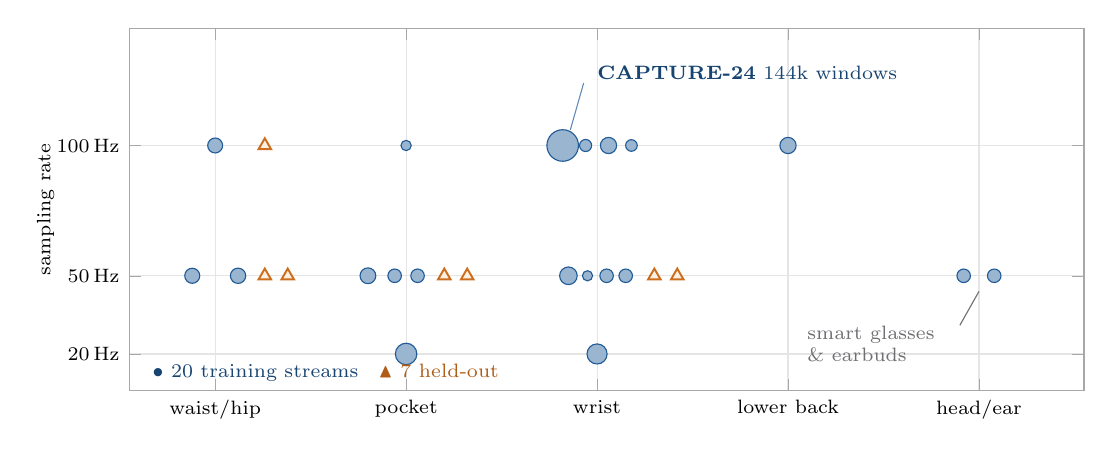
\begin{tikzpicture}
\begin{axis}[
  width=\columnwidth, height=4.6cm,
  xmin=0.55, xmax=5.55,
  ymin=6, ymax=145,
  ytick={20,50,100},
  yticklabels={20\,Hz,50\,Hz,100\,Hz},
  yticklabel style={font=\scriptsize},
  xtick={1,2,3,4,5},
  xticklabels={waist/hip,pocket,wrist,lower back,head/ear},
  xticklabel style={font=\scriptsize},
  ylabel={sampling rate},
  ylabel style={font=\scriptsize,yshift=-6pt},
  grid=major, grid style={draw=halogray!18},
  axis line style={draw=halogray!60},
  tick style={draw=halogray!60},
  scale only axis,
  clip=false,
]
% ---------- training streams (filled blue discs, diameter ~ #windows^0.4) ----
% diameters below are 2*(1.2 + 4.5*(n/144142)^0.4) pt, n = window count
\tikzset{hdisc/.style={circle,draw=haloblue,fill=haloblue!45,line width=0.4pt,inner sep=0pt}}
\node[hdisc,minimum size=5.44pt] at (axis cs:0.88,50)  {};% hhar        9,587
\node[hdisc,minimum size=5.40pt] at (axis cs:1.00,100) {};% kuhar       9,233
\node[hdisc,minimum size=5.54pt] at (axis cs:1.12,50)  {};% uci_har    10,299
\node[hdisc,minimum size=5.70pt] at (axis cs:1.80,50)  {};% unimib     11,771
\node[hdisc,minimum size=4.88pt] at (axis cs:1.94,50)  {};% xrf l.pkt   5,794
\node[hdisc,minimum size=7.76pt] at (axis cs:2.00,20)  {};% wisdm pkt  39,329
\node[hdisc,minimum size=4.88pt] at (axis cs:2.06,50)  {};% xrf r.pkt   5,794
\node[hdisc,minimum size=3.72pt] at (axis cs:2.00,100) {};% spsw pkt    1,179
\node[hdisc,minimum size=11.4pt] at (axis cs:2.82,100) {};% capture24 144,142
\node[hdisc,minimum size=6.36pt] at (axis cs:2.85,50)  {};% harmes     18,576
\node[hdisc,minimum size=4.36pt] at (axis cs:2.94,100) {};% pamap2      3,186
\node[hdisc,minimum size=3.68pt] at (axis cs:2.95,50)  {};% mhealth     1,104
\node[hdisc,minimum size=7.26pt] at (axis cs:3.00,20)  {};% wisdm wr   30,876
\node[hdisc,minimum size=4.88pt] at (axis cs:3.05,50)  {};% xrf l.wr    5,794
\node[hdisc,minimum size=5.86pt] at (axis cs:3.06,100) {};% nfi wrist  13,260
\node[hdisc,minimum size=4.88pt] at (axis cs:3.15,50)  {};% xrf r.wr    5,794
\node[hdisc,minimum size=4.20pt] at (axis cs:3.18,100) {};% spsw wrist  2,578
\node[hdisc,minimum size=5.86pt] at (axis cs:4.00,100) {};% nfi back   13,260
\node[hdisc,minimum size=4.88pt] at (axis cs:4.92,50)  {};% xrf glasses 5,794
\node[hdisc,minimum size=4.88pt] at (axis cs:5.08,50)  {};% xrf earbuds 5,794
% ---------- held-out datasets (open orange triangles) ----------
\addplot[only marks,mark=triangle*,mark size=2.6pt,color=haloorange,
         fill=halolight2,line width=0.7pt]
  coordinates {
    (1.26,50) (1.38,50) (1.26,100)
    (2.20,50) (2.32,50)
    (3.30,50) (3.42,50)
  };
% ---------- annotations ----------
\node[font=\scriptsize,color=haloblue!75!black,anchor=west] at (axis cs:2.95,128)
  {\textbf{CAPTURE-24} 144k windows};
\draw[haloblue!70,thin] (axis cs:2.86,106) -- (axis cs:2.93,124);
\node[font=\scriptsize,color=halogray,anchor=west,align=left] at (axis cs:4.05,24)
  {smart glasses\\ \& earbuds};
\draw[halogray,thin] (axis cs:5.00,44) -- (axis cs:4.90,31);
\node[font=\scriptsize,anchor=west,align=left] at (axis cs:0.62,13)
  {\textcolor{haloblue!75!black}{$\bullet$ 20 training streams}\;\;
   \textcolor{haloorange!85!black}{$\blacktriangle$ 7 held-out}};
\end{axis}
\end{tikzpicture}}
\caption{\textbf{The corpus does not cover a grid; it covers a scatter.} Each blue disc is
one of the 20 sensor streams HALO trains on, positioned by body placement and native
sampling rate, with area proportional to the number of $6$\,s windows it contributes; orange
triangles are the 7 held-out evaluation datasets. Rates span a $5\times$ range and placements
include two---smart glasses and wireless earbuds---that no established HAR benchmark
contains. Held-out cells are not simply new subjects: they combine placements and rates in
proportions the training corpus never sees. Absorbing this by resampling to a common rate
would discard the content above $10$\,Hz that only the $50$/$100$\,Hz streams can
resolve.}
\label{fig:corpus}

\end{figure}

\subsection{Inertial Signals Admit No Closed Grammar}
\label{sec:no_grammar}

The heterogeneity above is usually treated as an engineering nuisance to be absorbed by
pretraining on more of it. We think that is the wrong diagnosis, and the difference matters
because it changes what the solution has to be.

Foundation models in language and vision work in large part because their input space is
effectively \emph{closed} by a corpus. Text is produced by a grammar over a finite lexicon;
enough text does approach the distribution of sentences a model will meet. Natural images
obey a stable projective geometry and a stable statistics of surfaces and light. In both
cases the substrate has structure that a sufficiently large sample covers.

Inertial signals have no such closure. The map from a motion to a recorded signal is
composed at deployment time from a chain of choices---mounting orientation (a continuous
$SO(3)$ nuisance), body placement, sampling rate, filter chain, gravity convention, sensor
suite---and the chain composes. There is no finite enumeration to cover, and the free
parameters are continuous. A corpus $10\times$ larger reduces the \emph{probability} that a
new deployment is far from anything seen, but the tail does not close, and the transformations
that generate it are cheap to encounter: shipping on a second phone model, or a firmware
update, is enough.

If compatibility cannot come from coverage, it must come from \emph{inductive bias}: the
architecture, not the data, must make the representation invariant to the nuisance axes and
explicitly aware of the ones that carry signal. This is the standard move---but for inertial
sensing it has a failure mode on \emph{both} sides, and the interesting design question is
where to sit between them.

\textbf{Too much bias.} Layout-locked encoders fix a channel order, a channel count, and a
rate. They are the most sample-efficient thing to train and cannot read a device they were
not built for. Orientation-\emph{invariant} designs (e.g.\ training against uniformly
sampled $SO(3)$ rotations) are a subtler version of the same error: invariance is lossy.
Discarding orientation discards gravity, and with it the distinction between lying down and
standing still, which is exactly the kind of activity a posture or sleep application cares
about.

\textbf{Too little bias.} The opposite extreme treats every scalar channel as an independent
univariate series identified only by a free-text name. This is maximally flexible, and it
creates a shortcut. In a multi-corpus training set, the string describing a channel is
nearly a sufficient statistic for \emph{which corpus} the window came from; so is the
sampling rate, and so is the channel count. A model rewarded for predicting a label within a
corpus can satisfy much of that objective by first inferring the corpus and then predicting
its marginal---and cross-dataset evaluation is precisely where that strategy stops working.
We therefore treat corpus identifiability as a measurable failure and probe for it directly
(Table~\ref{tab:identity_probe}).

A third position, recently explored outside HAR, is to make the model \emph{equivariant} to
resolution---to condition its computation on the sampling rate so that it adapts, as in
sampling-rate-equivariant forecasting~\cite{flowstate} or grid-agnostic spectral
tokenization~\cite{spectraltok}. That is strictly better than resampling, but it is not the same
as what we want. An equivariant model still has to be \emph{told} the rate, and its features at
two rates are related by a learned transformation rather than being the same quantity. We want
the stronger property: that a feature \emph{denotes} a physical frequency, so a band computed
from a $20$\,Hz phone and a band computed from a $100$\,Hz research IMU are directly comparable
without any conditioning at all---which is what makes them comparable in a shared memory. Within
IMU sensing this property is, as far as we know, unclaimed: the closest tokenizer,
MoPFormer~\cite{mopformer}, resamples every dataset to $100$\,Hz before quantising into motion
primitives, so its codebook is defined over a fixed-rate grid.

The calibrated position, which HALO adopts, is to commit to the physics that does not vary
and to nothing that does. Three things do not vary: co-located axes on one rigid device
share a coordinate frame and must be rotated together, not independently; human motion
energy lives at physical frequencies, so a band means the same thing at every sampling rate;
and the quasi-static component of an accelerometer is gravity, so it carries posture and must
be preserved as a signed quantity rather than normalised away. Everything else---rate,
channel count, ordering, placement, which sensors exist---is deferred to run time and
described in language, at the granularity of the \emph{sensor} rather than the channel, so
that the description is expressive enough to name an unseen device but too coarse to
fingerprint a corpus.

\subsection{Sensor Similarity Does Not Track Linguistic Similarity}
\label{sec:geometry}

The second obstacle concerns the output side. Because deployments name their own activities,
a reusable model cannot have a fixed output layer, and the field's answer has been to embed
label strings with a frozen sentence encoder and align sensor features to that space, so
that recognition becomes nearest-neighbour retrieval over an arbitrary label
library~\cite{clip,lanhar,goat,unimts}. The mechanism is elegant and its premise is rarely
stated: that proximity in sentence-embedding space is a usable proxy for proximity in motion
space.

% =====================================================================
% fig_geometry.tex  --  L2 evidence: sensor similarity != linguistic similarity
%
% DATA PROVENANCE: cosine similarities between all-MiniLM-L6-v2 sentence
% embeddings of the label strings, measured 2026-07-26 by
%   sentence_transformers.SentenceTransformer('all-MiniLM-L6-v2')
% with normalize_embeddings=True.  Raw values in the arrays below; the
% generating script and its JSON output are archived with the paper source.
% The MOTION grouping (same vs different physical motion) is our own
% judgement and is stated as such in the caption -- it is not measured.
% =====================================================================
\begin{figure}[t]
\centering
\setlength{\abovecaptionskip}{3pt}
\setlength{\belowcaptionskip}{-4pt}
\resizebox{\columnwidth}{!}{%
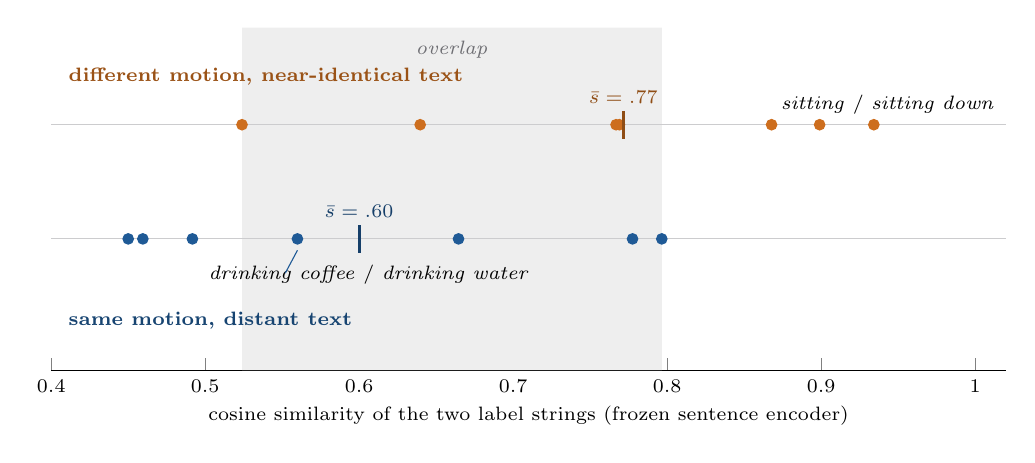
\begin{tikzpicture}
\begin{axis}[
  width=\columnwidth, height=4.35cm,
  xmin=0.40, xmax=1.02,
  ymin=-1.15, ymax=1.85,
  xtick={0.4,0.5,0.6,0.7,0.8,0.9,1.0},
  xticklabel style={font=\scriptsize},
  xlabel={cosine similarity of the two label strings (frozen sentence encoder)},
  xlabel style={font=\scriptsize,yshift=2pt},
  ytick={0,1},
  yticklabels={},
  axis y line=none,
  axis x line*=bottom,
  clip=false,
  scale only axis,
]
% ---- shaded overlap region: where the two groups interleave ----
\addplot[draw=none,fill=halogray!12,forget plot]
  coordinates {(0.5239,-1.15) (0.7965,-1.15) (0.7965,1.85) (0.5239,1.85)}
  \closedcycle;
\node[font=\scriptsize\itshape,halogray,anchor=south,align=center]
  at (axis cs:0.660,1.50) {overlap};

% ---- lane guides ----
\addplot[draw=halogray!35,thin,forget plot] coordinates {(0.40,1) (1.02,1)};
\addplot[draw=halogray!35,thin,forget plot] coordinates {(0.40,0) (1.02,0)};

% ---- TOP LANE: DIFFERENT physical motion, near-identical text ----
\addplot[only marks,mark=*,mark size=1.9pt,color=haloorange,forget plot]
  coordinates {(0.5239,1) (0.6396,1) (0.7668,1) (0.7690,1) (0.8678,1) (0.8990,1) (0.9342,1)};
% group mean
\addplot[only marks,mark=|,mark size=5pt,line width=1.1pt,color=haloorange!70!black,forget plot]
  coordinates {(0.7715,1)};

% ---- BOTTOM LANE: SAME physical motion, distant text ----
\addplot[only marks,mark=*,mark size=1.9pt,color=haloblue,forget plot]
  coordinates {(0.4500,0) (0.4595,0) (0.4917,0) (0.5599,0) (0.6645,0) (0.7775,0) (0.7965,0)};
\addplot[only marks,mark=|,mark size=5pt,line width=1.1pt,color=haloblue!70!black,forget plot]
  coordinates {(0.5999,0)};

% ---- lane titles ----
\node[font=\scriptsize\bfseries,color=haloorange!75!black,anchor=west]
  at (axis cs:0.405,1.42) {different motion, near-identical text};
\node[font=\scriptsize\bfseries,color=haloblue!75!black,anchor=west]
  at (axis cs:0.405,-0.72) {same motion, distant text};

% ---- callouts on the two headline pairs ----
\node[font=\scriptsize,anchor=south east,inner sep=1pt]
  (sitdown) at (axis cs:1.015,1.06) {\emph{sitting} / \emph{sitting down}};
\node[font=\scriptsize,anchor=north west,inner sep=1pt]
  (coffee) at (axis cs:0.500,-0.20) {\emph{drinking coffee} / \emph{drinking water}};
\draw[haloblue,thin] (axis cs:0.5599,-0.10) -- (axis cs:0.552,-0.30);

% ---- mean labels ----
\node[font=\scriptsize,color=haloorange!70!black,anchor=south] at (axis cs:0.7715,1.10) {$\bar{s}=.77$};
\node[font=\scriptsize,color=haloblue!70!black,anchor=south]   at (axis cs:0.5999,0.10) {$\bar{s}=.60$};
\end{axis}
\end{tikzpicture}}
\caption{\textbf{Sensor similarity and linguistic similarity are inverted, not merely
noisy.} Each dot is one pair of activity names from our label vocabulary, placed at the
cosine similarity of their frozen sentence embeddings (all-MiniLM-L6-v2, the encoder
language-aligned HAR models use). Pairs in the \emph{top} lane denote physically distinct
activities; pairs in the \emph{bottom} lane denote the same physical motion. If text
similarity tracked sensor similarity the lanes would separate, with the bottom lane on the
right. They separate the wrong way: the mean of the physically \emph{distinct} pairs
($0.77$) exceeds the mean of the physically \emph{identical} pairs ($0.60$), and $38$ of the
$49$ cross-lane comparisons are inverted. The motion grouping is our judgement; the
similarities are measured. A single projection from sensor space into this text geometry is
therefore mis-specified---which is why HALO retrieves in sensor space and votes in label
space (Section~\ref{sec:evidence_design}).}
\label{fig:geometry}
\end{figure}


It is not. Figure~\ref{fig:geometry} measures this on our own vocabulary. We selected $14$
label pairs---seven where the two names denote the same physical motion, seven where they
denote different motions---and computed the cosine similarity of their embeddings under
all-MiniLM-L6-v2, the encoder these systems use. If the premise held, the same-motion pairs
would sit to the right of the different-motion pairs. The ordering is reversed: the
different-motion pairs average $0.77$ and the same-motion pairs $0.60$, and $38$ of the $49$
cross-comparisons are individually inverted. \emph{Drinking coffee} and \emph{drinking
water} are the same wrist trajectory at $0.56$; \emph{sitting} and \emph{sitting down}, a
static posture versus a dynamic transition, are at $0.93$.

The failure is structural rather than a deficiency of one sentence encoder. Natural language
encodes activities by their \emph{object and purpose}---what is being drunk, what is being
cut---while an IMU sees only the \emph{kinematics of the limb}, which is invariant to the
object. Conversely, morphological relatives (\emph{sit}/\emph{sit down},
\emph{upstairs}/\emph{downstairs}) share nearly all of their surface form while denoting
opposite dynamics. No amount of alignment training repairs a target geometry that is wrong;
a model forced to fit it will minimise its loss by other means, and within a multi-dataset
corpus the cheapest other means is dataset identity.

The architectural consequence is to stop trying. HALO keeps language as the \emph{interface}
for naming activities---that part is necessary, and cheap---but does not use it as the
\emph{metric space} in which recognition happens. Retrieval is performed in sensor space,
where similarity means kinematic similarity; label text enters only afterwards, to name the
retrieved neighbours and to enumerate what the deployment is willing to predict
(Section~\ref{sec:evidence_design}).

\subsection{Design Requirements}
\label{sec:requirements}

The three claims yield four requirements.

\textbf{R1 (from L1).} The encoder must accept arbitrary sampling rates, channel counts,
sensor suites, and placements with one weight set and no architectural change, absorbing them
through construction rather than through resampling or per-dataset heads---and must signal
what a given configuration could not observe instead of silently fabricating it.

\textbf{R2 (from L1).} The conditioning that carries acquisition context must generalise
compositionally to unseen configurations, and must be coarse enough that it cannot serve as
a corpus identifier. This is a testable property, not an assertion.

\textbf{R3 (from L2).} Recognition over a run-time-declared label set must not require a
single projection reconciling sensor geometry with sentence geometry. Similarity must be
computed where it is meaningful, and label text used only where it is meaningful.

\textbf{R4 (from L3).} The model must place no floor on how much target supervision is
required, and adding a small amount must be possible without a gradient update, without
retraining, and without data leaving the device---so that $k{=}0$, $k{=}10$, and full
supervision are points on one curve rather than three different systems.

HALO meets R1--R2 with the physical-frequency filterbank tokenizer and factored per-sensor
language conditioning (Section~\ref{sec:tokenizer_design}), R3 with the evidence engine
(Section~\ref{sec:evidence_design}), and R4 because the evidence engine's memory is
append-only (Section~\ref{sec:deployment}).

% =========================
% 5_design.tex  --- calibrated tokenizer + label-free Phase A + evidence engine
% =========================
\section{Design of HALO}
\label{sec:design}

\subsection{System Overview}
\label{sec:overview}
\label{sec:requirements}

HALO is organised as two phases with a hard boundary (Figure~\ref{fig:overview}).
\textbf{Phase~A} learns a representation using no activity labels whatsoever; \textbf{Phase~B}
turns that frozen representation into a recogniser for whatever label set a deployment declares,
using labels only as annotations on stored exemplars. The boundary is where the argument of
Section~\ref{sec:motivation} lands: L1 says compatibility must be structural, so it belongs in
the encoder before any label is involved; L2 says the label decision must not be a projection
into text space, so it belongs after the encoder, in a component swappable per deployment.

\begin{figure*}[t]
    \centering
    \setlength{\abovecaptionskip}{4pt}
    \setlength{\belowcaptionskip}{-6pt}
  % PLACEHOLDER --- the system-overview figure is STALE and has been withdrawn from the manuscript.
%
% Why: the previous drawing labelled the encoder "two resolutions" and the loss box
% "masked latent + descriptor prediction". Both describe the pinned v2 artifact. The current
% repository default is a single fixed 1.0 s patch grid (multiresolution=False) with the
% descriptor term disabled (descriptor_weight=0), so the drawing no longer depicts the system.
%
% The previous TikZ source is preserved verbatim in figures/fig_overview_v2artifact.tex.
% Redraw from it once the checkpoint repin is decided. See STALENESS.md sec. 0 and sec. 2.
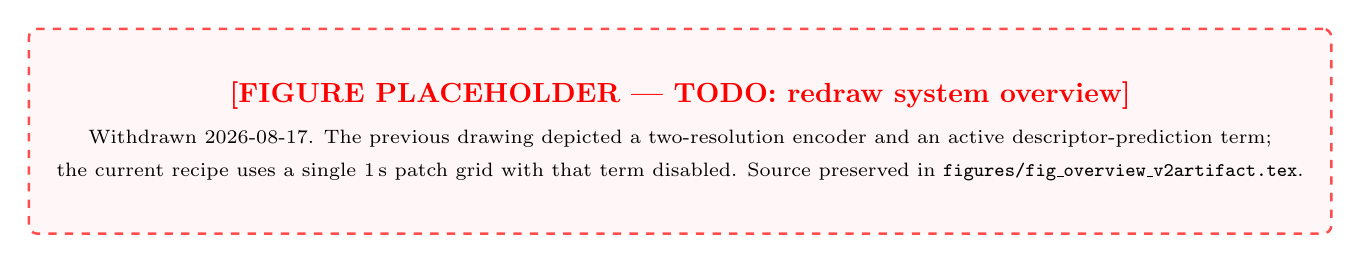
\begin{tikzpicture}
\node[draw=red!70,line width=0.9pt,dashed,rounded corners=3pt,inner sep=10pt,
      minimum width=0.96\textwidth,minimum height=26mm,align=center,fill=red!3]
  {\TODO{\textbf{[FIGURE PLACEHOLDER --- TODO: redraw system overview]}}\\[3pt]
   \scriptsize Withdrawn 2026-08-17. The previous drawing depicted a two-resolution encoder and an
   active descriptor-prediction term;\\
   \scriptsize the current recipe uses a single 1\,s patch grid with that term disabled.
   Source preserved in \texttt{figures/fig\_overview\_v2artifact.tex}.};
\end{tikzpicture}

  \caption{\textbf{HALO end to end.} One left-to-right path. Phase~A trains the tokenizer and
  encoder with objectives that never see an activity label. The encoder is then frozen and
  crosses the boundary unchanged---it is the \emph{same} weights that encode a query and that
  encoded every exemplar in memory, which is what lets the two be compared as vectors. Phase~B
  adds no parameters to that path: it appends encoded exemplars to a memory and accumulates
  evidence for the label strings declared at run time. Adding an activity, a placement, or a
  device is an append; no gradient step occurs anywhere to the right of \textsf{freeze}.}
  \label{fig:overview}
\end{figure*}

\textbf{One window, end to end.} A deployment hands HALO a $6$\,s window from whatever sensors it
has---say a $50$\,Hz watch accelerometer and gyroscope, six channels---plus one description string
per sensor and its list of activity names. The tokenizer cuts each channel into patches and turns
each patch into one token: a $32$-band constant-$Q$ readout on a frequency axis fixed in Hz, a
signed DC term carrying gravity, and two masks recording which of the $32$ bands this rate and
patch length could actually resolve. Nothing is resampled, so band $k$ denotes the same physical
frequency whether the device ran at $20$ or $100$\,Hz. Each token is then biased by the sentence
embedding of its sensor's description, and the token set---unordered over channels, positioned in
physical time---enters a $7.17$M-parameter transformer that emits one vector per patch. Those
vectors are the interface between the phases: Phase~A shapes them with objectives that never see
a label, and Phase~B compares them, by cosine similarity in that same space, against a memory of
encoded exemplars, accumulating evidence for whichever activity names were declared. The
demands of Section~\ref{sec:why} map onto this path one-to-one, and
Table~\ref{tab:mechanisms} fixes the name we use for each mechanism throughout. The distinctions
those names carry are the contribution: not ``a spectral tokenizer'' but one anchored to
\emph{physical} Hz; not a Nyquist mask but one bounded by the \emph{acquisition} clock; not
per-channel text but per-\emph{sensor}; not retrieval in CLIP space but in \emph{sensor} space.

\begin{table}[t]
  \centering
  \caption{Each deployment demand, the mechanism that answers it, and the name used for that
  mechanism throughout this paper. The qualifiers are load-bearing: each marks where HALO departs
  from the nearest existing technique. Rows 1--3 are the tokenizer
  (Section~\ref{sec:tokenizer_design}) and are what let one weight set accept any rate, channel
  count, and placement with no architectural change; rows 4--5 are the evidence engine
  (Section~\ref{sec:evidence_design}). Row 3 states a property we \emph{probe} rather than assert
  (Table~\ref{tab:tokenizer_ablation}), and row 5 is why no label budget requires a gradient
  update.}
  \label{tab:mechanisms}
  \scriptsize
  \setlength{\tabcolsep}{3pt}
  \begin{tabular}{@{}p{0.30\columnwidth} p{0.38\columnwidth} p{0.24\columnwidth}@{}}
    \toprule
    Demand & Mechanism & Name \\
    \midrule
    Rate and anti-aliasing differ per device
      & constant-$Q$ filterbank on a fixed physical-frequency axis over a native-rate transform;
        no resampling anywhere in the path
      & \textbf{physical-Hz tokenizer} \\[2pt]
    What a device \emph{could} measure differs
      & per-token masks bounded by the \textsc{acquisition} clock, not the rate the grid happens
        to be stored at
      & \textbf{acquisition-bounded observability masks} \\[2pt]
    Channel count, order and placement differ
      & free-text identity attached to the \textsc{sensor}, leaving channel count and order free
        while staying too coarse to fingerprint a corpus
      & \textbf{per-sensor language conditioning} \\[2pt]
    The label set belongs to the deployment
      & retrieve encoded exemplars by \textsc{sensor} similarity; accumulate evidence for whatever
        strings are declared at run time
      & \textbf{evidence retrieval in sensor space} \\[2pt]
    The label budget is small and fixed
      & append exemplars to memory; no gradient update at any budget
      & \textbf{append-only memory} \\
    \bottomrule
  \end{tabular}
\end{table}

\subsection{The Physical-Hz Tokenizer}
\label{sec:tokenizer_design}

\subsubsection{Per-sensor language conditioning: sensors, not channels}
\label{sec:sensor_grouping}

HALO's first commitment is that the unit of description is the \emph{sensor}, not the scalar
channel. Three co-located accelerometer axes share a coordinate frame: they rotate together,
experience the same gravity vector, and no physically realisable transformation moves one without
the others. Treating them as independent series discards this and lets per-channel text act as a
corpus fingerprint. HALO therefore models a stream as a \emph{set of sensors}, each a triad with
its own device, placement, and gravity convention---which also makes the augmentation physics
correct, since an $SO(3)$ rotation is applied jointly to a triad and its co-located gyroscope
rather than to a single axis.

Accelerometer streams are gravity-aware. The quasi-static component below the analysis band is
split off as a \emph{signed} per-axis DC feature rather than removed, so posture survives. On
$200$ real waist-phone windows each of standing, sitting and lying, the frequency path separates
no pair distinctly (all pairwise cosines within $0.84$--$0.88$) while signed DC places lying
nearly orthogonal to standing ($-0.04$); a design achieving orientation robustness through
\emph{invariance} discards that quantity, and with it the distinction between lying down
and standing still. Figure~\ref{fig:gravity} shows this and its
limit---standing and sitting stay at $0.99$ in DC, the same pair Section~\ref{sec:geometry} finds
inseparable in text, so neither path suffices alone. Because gravity conventions differ across
platforms, the convention is declared in the sensor's text and a gravity-removal augmentation is
applied with low probability, so the encoder sees both conventions for the same motion.

\subsubsection{A physical-frequency constant-$Q$ filterbank}
\label{sec:filterbank}

Each patch of each channel becomes one token entirely in the physical-frequency domain
(Appendix~\ref{app:tokenizer}, Figure~\ref{fig:tokenizer}). The patch is Hann-windowed and its DC
component removed, then
transformed by a zero-padded real DFT of fixed length $S{=}256$. The zero-padding is what makes
this rate-agnostic: for a patch sampled at rate $r$, DFT bin $m$ corresponds to physical frequency
$\phi[m] = mr/S$, so the \emph{same} matrix of bin indices maps to different Hz grids at different
rates, and the readout can be defined once in Hz. That readout is a constant-$Q$ Gaussian
filterbank~\cite{constantq,constantqfast} with $K{=}32$ centres log-spaced over $[0.3,15]$\,Hz at
$Q{=}4$. The limits are physical rather than tuned: gait cadence occupies $0.5$--$3$\,Hz, limb and
hand motion add harmonics to roughly $10$--$12$\,Hz, and content below $0.3$\,Hz is gravity, which
the signed DC feature already carries.

Rate-invariance is therefore a property of the construction rather than of a learned
approximation: a $2$\,Hz gait rhythm deposits energy in the same band whether the device sampled
at $20$ or $100$\,Hz, and because no interpolation exists in the path there is no aliasing to
introduce and no fabricated sample to explain away (Figure~\ref{fig:rateinv}). This is the
property, argued in Section~\ref{sec:no_grammar}, that rate-\emph{equivariance}~\cite{flowstate}
does not provide and that one flat cross-device memory requires.
Appendix~\ref{app:tokenizer} records the DFT- and patch-length guardrails.

\begin{figure*}[t]
    \centering
    \setlength{\abovecaptionskip}{4pt}
    \setlength{\belowcaptionskip}{-4pt}
  % =====================================================================
% fig_rateinvariance.tex --- L1 demonstrated on real data, not asserted.
%
% PROVENANCE: one 1.5 s accelerometer patch (x-axis) of `walking` from the
% NFI-FARED wrist stream, native 100 Hz, taken straight from the materialised
% native grid.  It is anti-alias resampled to 50 and 20 Hz with the same
% scipy.signal.resample_poly the data pipeline uses, then each version is run
% through the REAL PhysicalFilterbankTokenizer DSP path at ITS OWN rate
% (_spectral_power -> _apply_filterbank -> _observability_masks), exactly as in
% training.  Numbers generated 2026-07-26; cosines quoted in the caption are
% measured, not estimated.
% =====================================================================
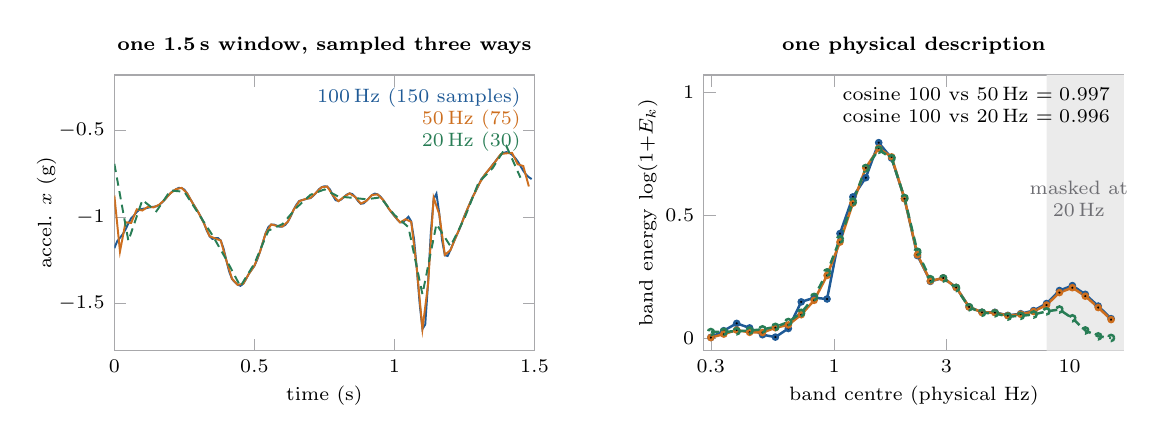
\begin{tikzpicture}

% ---------------- LEFT: the same motion, three different arrays -------------
\begin{axis}[
  name=sigax,
  width=0.44\textwidth, height=3.5cm,
  xmin=0, xmax=1.5, ymin=-1.77, ymax=-0.18,
  xlabel={time (s)}, ylabel={accel. $x$ (g)},
  xlabel style={font=\scriptsize,yshift=2pt}, ylabel style={font=\scriptsize,yshift=-6pt},
  xticklabel style={font=\scriptsize}, yticklabel style={font=\scriptsize},
  axis line style={draw=halogray!60}, tick style={draw=halogray!60},
  title={\scriptsize\bfseries one 1.5\,s window, sampled three ways},
  title style={yshift=-2pt},
  scale only axis,
]
\addplot[draw=haloblue,line width=0.7pt] coordinates {(0.0000,-1.1792) (0.0100,-1.1394) (0.0200,-1.1194) (0.0300,-1.0986) (0.0400,-1.0708) (0.0500,-1.0366) (0.0600,-1.0066) (0.0700,-0.9902) (0.0800,-0.9707) (0.0900,-0.9561) (0.1000,-0.9524) (0.1100,-0.9502) (0.1200,-0.9458) (0.1300,-0.9424) (0.1400,-0.9404) (0.1500,-0.9377) (0.1600,-0.9299) (0.1700,-0.9158) (0.1800,-0.8989) (0.1900,-0.8796) (0.2000,-0.8623) (0.2100,-0.8489) (0.2200,-0.8398) (0.2300,-0.8318) (0.2400,-0.8323) (0.2500,-0.8416) (0.2600,-0.8640) (0.2700,-0.8933) (0.2800,-0.9204) (0.2900,-0.9470) (0.3000,-0.9734) (0.3100,-1.0027) (0.3200,-1.0342) (0.3300,-1.0784) (0.3400,-1.1106) (0.3500,-1.1260) (0.3600,-1.1213) (0.3700,-1.1206) (0.3800,-1.1357) (0.3900,-1.1826) (0.4000,-1.2510) (0.4100,-1.3142) (0.4200,-1.3569) (0.4300,-1.3755) (0.4400,-1.3899) (0.4500,-1.3965) (0.4600,-1.3850) (0.4700,-1.3582) (0.4800,-1.3274) (0.4900,-1.3040) (0.5000,-1.2817) (0.5100,-1.2454) (0.5200,-1.1995) (0.5300,-1.1467) (0.5400,-1.0938) (0.5500,-1.0571) (0.5600,-1.0432) (0.5700,-1.0430) (0.5800,-1.0503) (0.5900,-1.0557) (0.6000,-1.0542) (0.6100,-1.0457) (0.6200,-1.0251) (0.6300,-0.9944) (0.6400,-0.9580) (0.6500,-0.9282) (0.6600,-0.9070) (0.6700,-0.9019) (0.6800,-0.8979) (0.6900,-0.8923) (0.7000,-0.8909) (0.7100,-0.8772) (0.7200,-0.8604) (0.7300,-0.8403) (0.7400,-0.8276) (0.7500,-0.8223) (0.7600,-0.8240) (0.7700,-0.8408) (0.7800,-0.8755) (0.7900,-0.9023) (0.8000,-0.9067) (0.8100,-0.8982) (0.8200,-0.8843) (0.8300,-0.8699) (0.8400,-0.8630) (0.8500,-0.8674) (0.8600,-0.8838) (0.8700,-0.9072) (0.8800,-0.9233) (0.8900,-0.9204) (0.9000,-0.9060) (0.9100,-0.8892) (0.9200,-0.8730) (0.9300,-0.8643) (0.9400,-0.8694) (0.9500,-0.8816) (0.9600,-0.9019) (0.9700,-0.9258) (0.9800,-0.9521) (0.9900,-0.9736) (1.0000,-0.9937) (1.0100,-1.0134) (1.0200,-1.0293) (1.0300,-1.0312) (1.0400,-1.0139) (1.0500,-0.9980) (1.0600,-1.0251) (1.0700,-1.1274) (1.0800,-1.2998) (1.0900,-1.4985) (1.1000,-1.6453) (1.1100,-1.6199) (1.1200,-1.3831) (1.1300,-1.0862) (1.1400,-0.8962) (1.1500,-0.8650) (1.1600,-0.9775) (1.1700,-1.1323) (1.1800,-1.2200) (1.1900,-1.2244) (1.2000,-1.1899) (1.2100,-1.1501) (1.2200,-1.1123) (1.2300,-1.0776) (1.2400,-1.0371) (1.2500,-0.9929) (1.2600,-0.9565) (1.2700,-0.9180) (1.2800,-0.8809) (1.2900,-0.8511) (1.3000,-0.8179) (1.3100,-0.7820) (1.3200,-0.7617) (1.3300,-0.7405) (1.3400,-0.7219) (1.3500,-0.6995) (1.3600,-0.6792) (1.3700,-0.6575) (1.3800,-0.6394) (1.3900,-0.6296) (1.4000,-0.6252) (1.4100,-0.6289) (1.4200,-0.6401) (1.4300,-0.6565) (1.4400,-0.6780) (1.4500,-0.7051) (1.4600,-0.7327) (1.4700,-0.7549) (1.4800,-0.7700) (1.4900,-0.7808)};
\addplot[draw=haloorange,line width=0.7pt] coordinates {(0.0000,-0.8758) (0.0200,-1.1987) (0.0400,-1.0296) (0.0600,-1.0337) (0.0800,-0.9552) (0.1000,-0.9619) (0.1200,-0.9404) (0.1400,-0.9440) (0.1600,-0.9283) (0.1800,-0.8995) (0.2000,-0.8624) (0.2200,-0.8390) (0.2400,-0.8315) (0.2600,-0.8639) (0.2800,-0.9210) (0.3000,-0.9728) (0.3200,-1.0368) (0.3400,-1.1104) (0.3600,-1.1233) (0.3800,-1.1355) (0.4000,-1.2514) (0.4200,-1.3555) (0.4400,-1.3905) (0.4600,-1.3852) (0.4800,-1.3284) (0.5000,-1.2804) (0.5200,-1.2001) (0.5400,-1.0942) (0.5600,-1.0423) (0.5800,-1.0505) (0.6000,-1.0544) (0.6200,-1.0255) (0.6400,-0.9579) (0.6600,-0.9088) (0.6800,-0.8969) (0.7000,-0.8894) (0.7200,-0.8594) (0.7400,-0.8280) (0.7600,-0.8236) (0.7800,-0.8744) (0.8000,-0.9082) (0.8200,-0.8831) (0.8400,-0.8632) (0.8600,-0.8842) (0.8800,-0.9222) (0.9000,-0.9065) (0.9200,-0.8726) (0.9400,-0.8688) (0.9600,-0.9014) (0.9800,-0.9520) (1.0000,-0.9928) (1.0200,-1.0307) (1.0400,-1.0121) (1.0600,-1.0277) (1.0800,-1.2972) (1.1000,-1.6461) (1.1200,-1.3882) (1.1400,-0.8884) (1.1600,-0.9829) (1.1800,-1.2179) (1.2000,-1.1908) (1.2200,-1.1131) (1.2400,-1.0370) (1.2600,-0.9546) (1.2800,-0.8833) (1.3000,-0.8159) (1.3200,-0.7607) (1.3400,-0.7204) (1.3600,-0.6809) (1.3800,-0.6360) (1.4000,-0.6320) (1.4200,-0.6294) (1.4400,-0.6949) (1.4600,-0.7054) (1.4800,-0.8232)};
\addplot[draw=halogreen,line width=0.7pt,densely dashed] coordinates {(0.0000,-0.6931) (0.0500,-1.1371) (0.1000,-0.9014) (0.1500,-0.9665) (0.2000,-0.8467) (0.2500,-0.8539) (0.3000,-0.9795) (0.3500,-1.1043) (0.4000,-1.2465) (0.4500,-1.3997) (0.5000,-1.2680) (0.5500,-1.0783) (0.6000,-1.0404) (0.6500,-0.9462) (0.7000,-0.8717) (0.7500,-0.8405) (0.8000,-0.8816) (0.8500,-0.8887) (0.9000,-0.8972) (0.9500,-0.8864) (1.0000,-0.9876) (1.0500,-1.0581) (1.1000,-1.4454) (1.1500,-1.0402) (1.2000,-1.1681) (1.2500,-1.0076) (1.3000,-0.8021) (1.3500,-0.7190) (1.4000,-0.5914) (1.4500,-0.7724)};
\node[font=\scriptsize,anchor=north east,align=right] at (rel axis cs:0.99,0.99)
  {\textcolor{haloblue}{100\,Hz (150 samples)}\\
   \textcolor{haloorange}{50\,Hz (75)}\\
   \textcolor{halogreen}{20\,Hz (30)}};
\end{axis}

% ---------------- RIGHT: one physical description ---------------------------
\begin{axis}[
  at={(sigax.right of east)}, anchor=left of west, xshift=9mm,
  width=0.44\textwidth, height=3.5cm,
  xmode=log, log basis x=10,
  xmin=0.28, xmax=17, ymin=-0.05, ymax=1.07,
  xtick={0.3,1,3,10}, xticklabels={0.3,1,3,10},
  xlabel={band centre (physical Hz)}, ylabel={band energy $\log(1{+}E_k)$},
  xlabel style={font=\scriptsize,yshift=2pt}, ylabel style={font=\scriptsize,yshift=-4pt},
  xticklabel style={font=\scriptsize}, yticklabel style={font=\scriptsize},
  axis line style={draw=halogray!60}, tick style={draw=halogray!60},
  title={\scriptsize\bfseries one physical description},
  title style={yshift=-2pt},
  scale only axis, clip=false,
]
% region the 20 Hz stream cannot legally observe
\addplot[draw=none,fill=halogray!14,forget plot]
  coordinates {(7.981,-0.05) (17,-0.05) (17,1.07) (7.981,1.07)} \closedcycle;
\node[font=\scriptsize,color=halogray,anchor=north,align=center]
  at (axis cs:10.94,0.68) {masked at\\ 20\,Hz};

\addplot[draw=haloblue,line width=0.9pt,mark=*,mark size=0.9pt] coordinates {(0.3000,0.0034) (0.3404,0.0307) (0.3861,0.0605) (0.4381,0.0421) (0.4970,0.0144) (0.5638,0.0047) (0.6397,0.0397) (0.7257,0.1478) (0.8233,0.1646) (0.9341,0.1595) (1.0597,0.4254) (1.2022,0.5744) (1.3639,0.6525) (1.5474,0.7949) (1.7555,0.7320) (1.9916,0.5676) (2.2595,0.3359) (2.5634,0.2311) (2.9082,0.2453) (3.2993,0.2069) (3.7431,0.1272) (4.2466,0.1056) (4.8177,0.1054) (5.4657,0.0930) (6.2009,0.0997) (7.0349,0.1124) (7.9811,0.1412) (9.0546,0.1939) (10.2725,0.2139) (11.6541,0.1785) (13.2217,0.1308) (15.0000,0.0796)};
\addplot[draw=haloorange,line width=0.9pt,mark=*,mark size=0.9pt] coordinates {(0.3000,0.0027) (0.3404,0.0169) (0.3861,0.0332) (0.4381,0.0241) (0.4970,0.0231) (0.5638,0.0429) (0.6397,0.0542) (0.7257,0.0957) (0.8233,0.1542) (0.9341,0.2553) (1.0597,0.3908) (1.2022,0.5489) (1.3639,0.6927) (1.5474,0.7722) (1.7555,0.7370) (1.9916,0.5670) (2.2595,0.3393) (2.5634,0.2328) (2.9082,0.2448) (3.2993,0.2065) (3.7431,0.1272) (4.2466,0.1051) (4.8177,0.1042) (5.4657,0.0917) (6.2009,0.0975) (7.0349,0.1085) (7.9811,0.1350) (9.0546,0.1856) (10.2725,0.2054) (11.6541,0.1710) (13.2217,0.1248) (15.0000,0.0757)};
\addplot[draw=halogreen,line width=0.9pt,densely dashed,mark=o,mark size=1.1pt] coordinates {(0.3000,0.0251) (0.3404,0.0265) (0.3861,0.0284) (0.4381,0.0312) (0.4970,0.0362) (0.5638,0.0462) (0.6397,0.0660) (0.7257,0.1034) (0.8233,0.1679) (0.9341,0.2677) (1.0597,0.4023) (1.2022,0.5552) (1.3639,0.6919) (1.5474,0.7660) (1.7555,0.7315) (1.9916,0.5699) (2.2595,0.3514) (2.5634,0.2399) (2.9082,0.2430) (3.2993,0.2041) (3.7431,0.1261) (4.2466,0.1034) (4.8177,0.1013) (5.4657,0.0879) (6.2009,0.0911) (7.0349,0.0964) (7.9811,0.1093) (9.0546,0.1168) (10.2725,0.0811) (11.6541,0.0317) (13.2217,0.0077) (15.0000,0.0013)};
\node[font=\scriptsize,anchor=north east,align=right] at (rel axis cs:0.99,0.99)
  {cosine $100$ vs $50$\,Hz $=0.997$\\ cosine $100$ vs $20$\,Hz $=0.996$};
\end{axis}
\end{tikzpicture}

  \caption{\textbf{Rate-invariance, measured rather than argued.} One $1.5$\,s wrist patch of
  \emph{walking} (NFI-FARED) anti-alias resampled to three rates and run through the tokenizer at
  each. \emph{Left:} as arrays these are three different objects---$150$, $75$ and $30$ numbers,
  no sample coinciding---so any encoder positioned by timestep index sees three different
  structures. \emph{Right:} the band energies coincide (cosine $0.997$ and $0.996$ over the $26$
  commonly observable bands). The shaded region is what $20$\,Hz physically cannot see: those
  bands are \emph{masked}, not estimated. The $20$\,Hz curve does fall away inside it---exactly
  the loss an encoder that resampled the whole corpus would silently take on every stream.}
  \label{fig:rateinv}
\end{figure*}

\subsubsection{Observability: say what could not be measured}
\label{sec:masks}

Rate-invariance would be dishonest without a second mechanism. A $20$\,Hz stream cannot report
energy at $12$\,Hz, and a $0.4$\,s patch cannot resolve a $0.3$\,Hz band. Rather than emitting a
small number the encoder might read as ``no energy here,'' each token carries two masks. The
\emph{Nyquist observability} mask marks band $k$ observable only if
$c_k + 2\sigma_k \le 0.9\,(r/2)$, a $10\%$ guard so a band's Gaussian tail does not straddle the
aliasing edge; the \emph{resolution} mask marks it resolved only if one full cycle fits in the
patch, $c_k \ge 1/D$ (Figure~\ref{fig:tokenizer}). A band that is present but blurry is flagged,
not zeroed, and streams resampled by their publisher take the Nyquist bound from the
\emph{acquisition} rate, since upsampling cannot create information.

\subsubsection{Factored language conditioning}
\label{sec:conditioning}

Tokens from a weight-shared tokenizer are agnostic to what produced them, so acquisition context
must be injected. HALO factors it in two: a \textbf{role} string per channel naming \emph{only}
the axis (\texttt{"x"}, \texttt{"y"}, \texttt{"z"}), constant across the corpus; and a
\textbf{sensor identity} string per sensor carrying device, modality, placement and gravity
convention, e.g.\ \texttt{"a smartwatch accelerometer on the wrist; includes gravity"}. Both are
embedded by the same frozen sentence encoder~\cite{sbert} and fused into the token, the sensor
embedding through a gated residual initialised near zero so conditioning starts as a gentle bias
and grows only if it earns its place.

The factorisation is the point: the description a channel receives is shared by every sensor of
that kind across the corpus, which is what makes it too coarse to identify a dataset. Numeric
metadata is deliberately \emph{absent}, because a frozen sentence encoder represents numbers
unreliably; rate and duration enter through the bin$\to$Hz map and the masks instead. Sensor
strings are paraphrased during training and sometimes dropped to a generic one, so the encoder
must tolerate an unfamiliar description at deployment. Whether this buys the anti-memorisation it
is designed for is empirical: Table~\ref{tab:tokenizer_ablation} tests it against
per-channel-text and layout-locked variants.

\subsubsection{Set encoder over physical time}
\label{sec:encoder}

Conditioned tokens enter a dual-branch transformer~\cite{transformer} alternating \emph{temporal}
self-attention within a channel and \emph{cross-channel} self-attention within a patch, with
channel masks so absent or padded channels never contribute. Channels carry no positional index
at all---their identity is text---so the encoder is permutation- and count-invariant over
channels by construction, and a device with three channels and one with twelve are the same kind
of input. Temporal positions use rotary embeddings~\cite{rope} keyed to \emph{physical time}
rather than patch index: the filterbank's counterpart on the time axis, so a $1.2$\,s gesture
receives the same relative code regardless of rate or patch length. The encoder is $7.17$M
trainable parameters ($d{=}256$, $6$ layers, $8$ heads) plus a frozen all-MiniLM-L6-v2 sentence
encoder ($22.7$M) shared by sensor conditioning and label text, reading $6$\,s windows tokenised
at two resolutions. Because rotary positions are relative and the tokenizer uses no cross-patch
statistics, offline and causal operation differ only by the attention mask and the encoder
implements both---an affordance, not a claim, since we do not measure a causal arm here.

\subsection{Phase A: Label-Free Pretraining of the Physical-Hz Tokenizer and Encoder}
\label{sec:phaseA_design}

Phase A trains the tokenizer and encoder with objectives that never observe an activity label.
This is a change of principle, not an economy: as long as the objective is closed-vocabulary
label prediction, the model is rewarded for exploiting whatever predicts labels within the
training corpora---the failure of Section~\ref{sec:no_grammar}---and removing labels also unlocks
unlabelled data, which is where the scale in wearables is (full spec in
Appendix~\ref{app:phasea}).

\textbf{(A1) Masked prediction, with two targets.} A validity-aware mask over physical-time
intervals hides a subset of tokens; at masked positions the encoder predicts both the \emph{fixed}
filterbank features of the hidden content and the \emph{contextual latents} a stop-gradient EMA
teacher~\cite{byol,data2vec,ijepa} produces from the unmasked window. The fixed target grounds
the representation in physical quantities; the latent target lets it become more abstract than
its own input features.

\textbf{(A2) VICReg over augmented views.} Two independently augmented views are pulled together
under VICReg~\cite{vicreg} rather than a contrastive loss, for a reason specific to this corpus:
NT-Xent declares the other windows in a batch negatives, and in a multi-dataset corpus the batch
is full of the same activity from other subjects and datasets, so it actively pushes apart things
that should be together. VICReg needs no negatives; SimCLR~\cite{simclr} and SupCon~\cite{supcon}
remain selectable as controls. Text augmentation uses a \emph{shared} seed across views, so a pair
never differs only in whether its configuration was described.

\textbf{(A3--A5) Three low-weight rails} complete the objective: time--frequency consistency
against an auxiliary time-domain encoder discarded at inference (inspired by TF-C~\cite{tfc} but
not faithful to it); a cross-placement term over \emph{verified simultaneous} recordings of one
physical event at two or more placements ($17{,}387$ paired events), whose positive identity
comes from explicit event identifiers written during conversion, never from array alignment or an
activity label; and two self-derived targets as a sanity anchor. Model selection uses
subject-disjoint $k$-NN accuracy---labels are a \emph{metric} here, never in the loss.

\subsection{Phase B: Evidence Retrieval in Sensor Space}
\label{sec:evidence_design}

The encoder is frozen. What remains is to turn its representation into a decision over label
strings supplied at run time, without the single sensor-to-text projection
Section~\ref{sec:geometry} showed to be mis-specified. Figure~\ref{fig:evidence} shows the
mechanism.

\begin{figure}[t]
    \centering
    \setlength{\abovecaptionskip}{4pt}
    \setlength{\belowcaptionskip}{-4pt}
  % =====================================================================
% fig_evidence.tex  --  how Phase B turns a frozen representation into a
% decision over run-time label strings.
%
% This is a MECHANISM diagram, not a data plot: every quantity in it is
% structural (which vector retrieves what, where label text enters, what
% the decoder emits).  Nothing here is a measurement; the three bars are
% illustrative and the caption says so.
%
% Layout discipline: four horizontal bands at fixed y, nothing floating.
% Natural width ~8.0cm against an 8.46cm column, so \resizebox scales up
% slightly.  Explanatory prose belongs in the caption.
% NOTE: keep every \\ at the top level of a node body.
% =====================================================================
\resizebox{\columnwidth}{!}{%
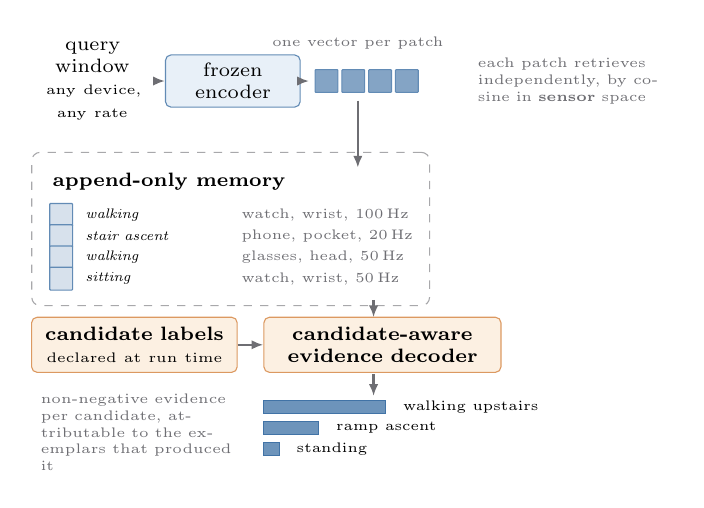
\begin{tikzpicture}[font=\scriptsize]

% ============ band 1: query -> one vector per patch ============
\node[hplain,anchor=west,text width=15mm] (qw) at (0,0)
  {query window\\ \tiny any device, any rate};
\node[hbox,anchor=west,text width=15mm,minimum height=6mm] (fe) at (1.75,0)
  {frozen encoder};
\foreach \i in {0,1,2,3} { \node[fbok,anchor=west] at (3.65+0.34*\i,0) {}; }
\node[font=\tiny,color=halogray,anchor=south] at (4.20,0.28) {one vector per patch};
\draw[harrow] (qw.east) -- (fe.west);
\draw[harrow] (fe.east) -- (3.58,0);

\node[font=\tiny,color=halogray,anchor=west,align=left,text width=24mm] at (5.60,0)
  {each patch retrieves independently, by cosine in \textbf{sensor} space};

% ============ band 2: one flat memory ============
\node[font=\scriptsize,anchor=west] (memtitle) at (0.20,-1.28)
  {\textbf{append-only memory}};
\foreach \i/\lab/\cfg in {%
  0/{\emph{walking}}/{watch, wrist, 100\,Hz},
  1/{\emph{stair ascent}}/{phone, pocket, 20\,Hz},
  2/{\emph{walking}}/{glasses, head, 50\,Hz},
  3/{\emph{sitting}}/{watch, wrist, 50\,Hz}} {
  \node[fbblur,anchor=west] (m\i) at (0.28,-1.70-0.27*\i) {};
  \node[font=\tiny,anchor=west] at (0.62,-1.70-0.27*\i) {\lab};
  \node[font=\tiny,color=halogray,anchor=west] (c\i) at (2.60,-1.70-0.27*\i) {\cfg};
}
\node[hphase,fit=(memtitle)(m0)(m3)(c0)(c3),inner sep=4pt] (mem) {};
\draw[harrow] (4.20,-0.25) -- (4.20,-1.10);

% ============ band 3: candidates enter, decoder decides ============
\node[hbox2,anchor=west,text width=24mm,minimum height=7mm] (cand) at (0.05,-3.35)
  {\textbf{candidate labels}\\ \tiny declared at run time};
\node[hbox2,anchor=west,text width=28mm,minimum height=7mm] (dec) at (3.00,-3.35)
  {\textbf{candidate-aware evidence decoder}};
\draw[harrow] (cand.east) -- (dec.west);
\draw[harrow] (4.40,-2.78) -- (4.40,-3.00);

% ============ band 4: non-negative evidence per candidate ============
% bars start BELOW the arrow tip -- an arrowhead landing inside bar 0 reads
% as if the decoder emitted only the first candidate.
\foreach \i/\lab/\w in {0/{walking upstairs}/1.55, 1/{ramp ascent}/0.70, 2/{standing}/0.20} {
  \fill[haloblue!65,draw=haloblue!85,line width=0.3pt]
    (3.00,-4.22-0.27*\i) rectangle ++(\w,0.17);
  \node[font=\tiny,anchor=west] at (3.10+\w,-4.135-0.27*\i) {\lab};
}
\draw[harrow] (4.40,-3.72) -- (4.40,-4.00);
\node[font=\tiny,color=halogray,anchor=west,align=left,text width=26mm] at (0.05,-4.46)
  {non-negative evidence per candidate, attributable to the exemplars that produced it};
\end{tikzpicture}}

  \caption{\textbf{How a decision is made without a sensor-to-text projection.} Each patch of the
  query retrieves independently, by cosine similarity in \emph{sensor} space, from one flat
  memory whose rows may come from any device---that is what physical-Hz anchoring buys, and it is
  what a resampling or rate-conditioned encoder cannot offer without a per-configuration index.
  Label text enters only twice, and never as a metric: to name what a neighbour was, and to
  enumerate what the deployment will accept as an answer. The decoder emits non-negative evidence
  per candidate, attributable to the exemplars that produced it. Structural diagram---the bar
  lengths are illustrative, not measured.}
  \label{fig:evidence}
\end{figure}

\textbf{Memory and retrieval.} Every labelled window available---from the training corpus and,
optionally, the target deployment---is encoded once and written to a versioned table storing the
patch vector with its label, subject, dataset, acquisition configuration, and source event. The
table is append-only: adding a class, a placement, or a device is a write, not a training run.
Every artifact is bound to the Phase-A checkpoint it was built from, and a behavioural probe
rejects a bank whose encoder has since changed---silently stale memory is the most dangerous
failure mode this design has. Each query patch then retrieves independently in \emph{sensor} space
under learned projections, each defining its own subspace and evidence contribution. During
training the query's own window, event, and subject are excluded, and contributions are capped per
source window and per label so one long recording cannot dominate a vote.

\textbf{Candidate-aware decoding.} Retrieved evidence is not simply averaged. A small set
transformer contextualises query and evidence tokens, refines each evidence item's label text as a
residual in frozen sentence space---which is what lets a neighbour labelled \emph{walking} but
retrieved in a stair-climbing context contribute as \emph{walking upstairs}---and pools evidence
as a residual on the retrieval prior. Candidate tokens carry frozen label text and attend
permutation-equivariantly over the evidence, so neither candidate nor evidence order carries
meaning. Every sublayer is gated by a LayerScale initialised near zero and the residuals are
zero-initialised, so at initialisation the decoder is \emph{exactly} the untrained
retrieval-plus-text-ensemble mechanism: every trained arm has an exact untrained control, reported
side by side.

\textbf{Confidence and rejection.} There is no \textsc{unknown} candidate; a rejection confidence
is estimated separately~\cite{selectiveclass,edl} from evidence mass, retrieval density,
agreement, and the leading margin, calibrated on truth-absent episodes with risk/coverage
reported---and truth-present episodes require support, so always-reject is not a solution.
Complete label \emph{families} are held out of decoder training for model selection
(Appendix~\ref{app:phaseb}).

\textbf{Deployment.}
\label{sec:deployment}%
A deployment is two pieces of configuration and no code: one description string per sensor and a
list of activity names, both embedded once and cached, so run-time cost is one encoder pass plus
a retrieval. The label-efficiency dial is the memory: at $k{=}0$ evidence comes from corpus
exemplars and candidate strings alone; at $k{>}0$ each demonstration costs one forward pass and
is immediately available---no gradient step, no revalidation, no requirement that data leave the
device. We expose this behind a small \texttt{predict()} interface and package the encoder for
Core~ML (Section~\ref{sec:case_study}).

% =========================
% 6_experiments.tex  --- protocol and tables written; result cells reserved (\PH / \PENDING)
% =========================
\section{Experiments}
\label{sec:experiments}

\PENDING{Corpus, protocol, and table structure are final; orange cells are reserved for results.}

\subsection{Methodology}
\label{sec:methodology}

We ask four questions. \textbf{(Q1)} Along the label-efficiency curve, where does HALO stand
against strong frozen encoders, and is there a regime it owns? \textbf{(Q2)} Does the tokenizer's
inductive bias do what Section~\ref{sec:no_grammar} claims---and, decisively, does anchoring let
one flat memory serve devices it was not built from? \textbf{(Q3)} Which Phase-A objectives carry
the transfer? \textbf{(Q4)} Does the system run on a phone?

\subsubsection{Data}
\label{sec:datasets}

We train on 12 public HAR datasets contributing 20 distinct sensor streams and evaluate on 7
never seen during training; Appendix~\ref{app:corpus} lists both with per-dataset rates,
placements, and window counts, and records the six datasets deliberately excluded and why. After
conversion to native-rate grids and removal of 95 windows exceeding physically possible sensor
rails, the corpus is $343{,}140$ non-overlapping six-second windows---$572$ hours---over $93$
labels, split subject-disjointly into $300{,}231$ training and $42{,}909$ validation windows, the
latter built by a greedy label-cover procedure so all $93$ labels are represented. Training rates
span $20$--$100$\,Hz over placements at the wrist, waist, pocket, lower back, ear, and head; the
held-out sets range from $1{,}260$ to $11{,}237$ windows over $6$ to $13$ labels.

\subsubsection{Baselines and the fairness contract}
\label{sec:baselines}

Cross-model comparison here is easy to get wrong, because the models do not accept the same
inputs. We state one contract and apply it uniformly (Appendix~\ref{app:baselines}): each model
occupies a \emph{level} on each of four tiers---architecture, rate, channels/placement, and label
vocabulary---and we never modify a released checkpoint's input contract, because doing so
discards the model being tested. CrossHAR and LiMU-BERT release no checkpoint compatible with our
corpus, so we pretrain them on \emph{our} data with their own published objectives, making their
data identical to ours; harnet, UniMTS and NormWear are used as released, which is faithful but
means their pretraining corpora differ from ours and from each other. This distinction is
material---harnet is pretrained on roughly $700$k person-days against our $572$
hours---and we state it wherever a comparison could be read as data-matched. Closed-vocabulary
models are bridged to arbitrary label strings with ConSE~\cite{conse}, so that ``can predict an
unseen label'' is available to every model and is not something HALO is credited for.

\subsubsection{Protocol}
\label{sec:eval_protocol}

\emph{Scoring.} Following the zero-shot evaluation literature~\cite{zslgbu}, every held-out
dataset is scored against its \emph{own} label strings, never a shared training-wide ontology, so
a prediction counts only if it retrieves that dataset's exact activity name. Macro-F1 is primary,
with accuracy alongside, because held-out label distributions are imbalanced.

\emph{Splits.} All few-shot fits and memory writes use subjects disjoint from those evaluated,
rotating over grouped folds with a confidence interval where a cohort is small enough that one
split is unstable. TNDA-HAR is distributed without per-window subject identifiers, so a
subject-disjoint boundary cannot be constructed for it; we report it separately and exclude it
from the subject-disjoint mean rather than implying a guarantee we cannot honour.

\emph{Label leakage.} The inference-time label-text ensemble is purged of synonyms drawn from the
evaluation datasets, so no evaluation vocabulary enters through paraphrase, and retrieval
hyper-parameters are selected on held-out \emph{training} configurations.

\emph{Parity control.} To separate the architecture from its native-rate and rich-text inputs,
HALO is also evaluated under baseline-equivalent inputs---$20$\,Hz resampling, neutral sensor
description---against the best member of each baseline group (Appendix~\ref{app:parity}).

\subsection{Q1: The Label-Efficiency Curve}
\label{sec:label_efficiency}

This is the headline experiment (Table~\ref{tab:label_efficiency}). At each budget $k$ of
labelled target windows per class we compare three mechanisms on identical data: HALO's memory, given the exemplars as an append with
\emph{no gradient update}; a probe on HALO's frozen features; and the same probe on frozen harnet
features. We additionally report \emph{retrieval over harnet features}---the same mechanism on a
different encoder---because without it a win could be credited to the mechanism when it belongs
to the representation, or the reverse.

The budget is reported in two units, because neither alone is honest: per-class $k$ is what a
deployment controls, while the fraction of the target dataset makes the numbers comparable to the
$1\%$/$5\%$/$10\%$ convention of the transfer literature. On our held-out sets the two coincide
closely---$k{=}10$ per class is $0.7$--$4.8\%$ of a dataset---and the grid stops at $k{=}100$
because beyond it the budget exceeds what the smaller sets contain.

\begin{table}[t]
  \centering
  \caption{Macro-F1 versus label budget, averaged over the held-out datasets, subject-disjoint
  throughout. $k{=}0$ is the zero-shot point and $k{=}\text{full}$ the supervised one; they are
  ends of one curve, not separate experiments, and every row uses \emph{one} frozen encoder
  across all $k$. The second header row converts $k$ into the mean fraction of a target dataset
  it represents. $^\dagger$\,The mechanism-versus-representation control: if retrieval helps only
  on HALO features the contribution is the encoder; if it helps equally on harnet's, it is the
  memory. We pre-register that we report this control regardless of which way it falls.}
  \label{tab:label_efficiency}
  \scriptsize
  \setlength{\tabcolsep}{1.5pt}
  \begin{tabular}{@{}l cccccc@{}}
    \toprule
    & \multicolumn{6}{c}{labelled target windows per class ($k$)} \\
    \cmidrule(lr){2-7}
    Mechanism & 0 & 5 & 10 & 25 & 100 & full \\
    \emph{(mean \% of target)} & \emph{0} & \emph{1.3} & \emph{2.7} & \emph{6.6} & \emph{27} & \emph{100} \\
    \midrule
    HALO memory (no gradient step)   & \PH & \PH & \PH & \PH & \PH & \PH \\
    HALO frozen $+$ probe            & \PH & \PH & \PH & \PH & \PH & \PH \\
    harnet frozen $+$ probe          & \PH & \PH & \PH & \PH & \PH & \PH \\
    harnet frozen $+$ memory\rlap{$^\dagger$} & \PH & \PH & \PH & \PH & \PH & \PH \\
    \midrule
    UniMTS (native text)             & \PH & \PH & \PH & \PH & \PH & \PH \\
    CrossHAR $+$ ConSE               & \PH & \PH & \PH & \PH & \PH & \PH \\
    LiMU-BERT $+$ ConSE              & \PH & \PH & \PH & \PH & \PH & \PH \\
    NormWear (native text)           & \PH & \PH & \PH & \PH & \PH & \PH \\
    \bottomrule
  \end{tabular}
\end{table}

\textbf{Pre-registered hypothesis and kill criterion.} We expect retrieval to win at small $k$,
where a nearest-neighbour decision beats a linear fit on a handful of points, and the probe to
overtake somewhere between $k{=}10$ and $k{=}25$---roughly the $3$--$7\%$ band. If that holds,
the regime HALO owns is $k \le 10$, which is the enrollment setting a user can perform in under a
minute. If the probe dominates at \emph{every} $k$ including the smallest, retrieval has no
regime of its own; we will report that outcome plainly. Appendix~\ref{app:perdataset} reports the
per-dataset breakdown, including InclusiveHAR stratified by ability, because a model that works
only for able-bodied users is not a foundation for rehabilitation applications.

\subsection{Q2: Does the Inductive Bias Do What It Claims?}
\label{sec:bias_experiments}

Section~\ref{sec:no_grammar} made two falsifiable claims about the tokenizer. Both are tested
directly rather than inferred from end-task accuracy.

\textbf{Rate-invariance is measured, not assumed.} A closed-form check confirms a pure tone
deposits identical band energies at $20$, $50$, and $100$\,Hz. The end-task version is
Table~\ref{tab:tokenizer_ablation}: the same encoder on the same data but reading a common
$20$\,Hz resampling of every stream. If the faster streams carry discriminative content above
$10$\,Hz, resampling must destroy it, and the gap measures how much.

\textbf{Does anchoring actually make one cross-device memory well-posed?} This experiment decides
whether HALO is an assembly of known parts or an enabling result. A flat memory shared across
devices is only meaningful if a query encoded from one configuration retrieves useful neighbours
stored from a \emph{different} one, which is what Table~\ref{tab:crossconfig} measures. The
measurement is unusually clean because parts of our corpus contain \emph{verified simultaneous}
recordings---the same person, activity, and instant, captured by two or more devices at different
placements---so querying one stream against a memory built only from its simultaneous partner
isolates configuration from subject, session, and activity entirely. We report the same matrix
for a resample-to-common-rate variant of our own encoder and for the frozen baselines, so the
comparison is of mechanisms rather than corpora.

\textbf{Is the naive assembly enough?} Since HALO's components have individually appeared before,
the claim that they must be assembled \emph{this particular way} is empirical.
Table~\ref{tab:tokenizer_ablation} includes the obvious alternative as a row: resample every
stream to a common rate, attach free text per channel, same retrieval on top. If that arm matches
HALO the architecture is a combination and we will say so; mutual entailment predicts it will
not, and predicts a reason---per-channel conditioning showing up as elevated dataset
identifiability, resampling as a rate gap.

\begin{table}[t]
  \centering
  \caption{\textbf{Cross-configuration retrieval: the enabling claim.} Each row queries with one
  acquisition configuration against a memory containing \emph{only} a different one. Because
  these pairs are verified simultaneous recordings, the only thing that varies is the
  configuration, so off-diagonal degradation is attributable to it alone. \emph{Retention} is
  cross divided by same: features that denote the same physical quantity across devices should
  retain most of their quality; one that resamples or conditions on the rate should not.}
  \label{tab:crossconfig}
  \scriptsize
  \setlength{\tabcolsep}{4pt}
  \begin{tabular}{@{}l cc cc@{}}
    \toprule
    & \multicolumn{2}{c}{HALO} & \multicolumn{2}{c}{resample-to-20\,Hz} \\
    \cmidrule(lr){2-3}\cmidrule(lr){4-5}
    Query $\rightarrow$ memory & same & \textbf{cross} & same & \textbf{cross} \\
    \midrule
    wrist $\rightarrow$ pocket (SP-SW-HAR)   & \PH & \PH & \PH & \PH \\
    wrist $\rightarrow$ lower back (NFI)     & \PH & \PH & \PH & \PH \\
    pocket $\rightarrow$ watch (WISDM)       & \PH & \PH & \PH & \PH \\
    wrist $\rightarrow$ ear/glasses (XRF~V2) & \PH & \PH & \PH & \PH \\
    100\,Hz $\rightarrow$ 20\,Hz memory      & \PH & \PH & \PH & \PH \\
    \midrule
    \textbf{cross/same retention}            & \multicolumn{2}{c}{\PH} & \multicolumn{2}{c}{\PH} \\
    \bottomrule
  \end{tabular}
\end{table}

\textbf{Conditioning must not be a corpus fingerprint.} The right-hand columns of
Table~\ref{tab:tokenizer_ablation} report a dataset-identity probe: a linear classifier fitted on
frozen embeddings of held-out subjects to predict which \emph{source dataset} a window came from.
A representation that has absorbed the acquisition description as a corpus identifier makes this
easy; one whose conditioning is genuinely compositional does not. It is the only direct evidence
we have for the ``too little bias'' failure mode, so we report it whether or not it favours us.

\begin{table}[t]
  \centering
  \caption{Tokenizer inductive-bias ablation (macro-F1 over the held-out datasets), each
  component removed independently, with the dataset-identity probe alongside. The
  \emph{naive assembly} row is not an ablation but a \emph{rival}: the same retrieval mechanism
  over an encoder built the conventional way. It is the arm that tests whether HALO is a
  combination of known parts. $^\ddagger$\,\emph{Rate gap} is performance on the $100$\,Hz
  held-out cell minus the same data downsampled to $20$\,Hz---what resampling costs.
  \emph{ds-ID} is dataset-identity accuracy; lower is better.}
  \label{tab:tokenizer_ablation}
  \scriptsize
  \setlength{\tabcolsep}{1.5pt}
  \begin{tabular}{@{}l cc cc@{}}
    \toprule
    & \multicolumn{2}{c}{transfer} & \multicolumn{2}{c}{probe} \\
    \cmidrule(lr){2-3}\cmidrule(lr){4-5}
    Tokenizer configuration & $k{=}0$ & $k{=}10$ & rate gap\rlap{$^\ddagger$} & ds-ID $\downarrow$ \\
    \midrule
    Physical-Hz, sensor-grouped, factored text & \PH & \PH & \PH & \PH \\
    \quad$-$ filterbank (resample to 20\,Hz)   & \PH & \PH & \PH & \PH \\
    \quad$-$ sensor grouping (per-chan.\ text) & \PH & \PH & \PH & \PH \\
    \quad$-$ language conditioning (locked)    & \PH & \PH & \PH & \PH \\
    \quad$-$ observability / resolution masks  & \PH & \PH & \PH & \PH \\
    \quad$-$ signed DC (gravity) feature       & \PH & \PH & \PH & \PH \\
    \midrule
    \emph{naive}: resample $+$ per-chan.\ text & \PH & \PH & \PH & \PH \\
    \midrule
    harnet~\cite{sslwearables} / UniMTS~\cite{unimts} & \PH & \PH & --- & \PH \\
    chance                                     & --- & --- & --- & \PH \\
    \bottomrule
  \end{tabular}
\end{table}

\subsection{Q3: Which Phase-A Objectives Carry the Transfer?}
\label{sec:objective_ablation}

Each Phase-A term is removed independently with all others held fixed
(Appendix~\ref{app:objectives}). Two controls matter more than the ablation itself. The
\emph{untrained control}: the decoder is identity-at-initialisation by construction, so every
trained arm is reported against the same architecture untrained, and a component that does not
beat its own initialisation is reported as such. The \emph{label-supervised control}: the
original supervised recipe remains selectable, so the claim that going label-free helps is
measured, not asserted.

\subsection{Q4: On-Device Cost and a Real Deployment}
\label{sec:deployment_experiments}
\label{sec:case_study}

We implement the full pipeline as an iOS application and will report encoder latency and peak
memory under Core~ML, retrieval latency against bank size, and a case study in which a user
enrolls activities by demonstration, changes body placement mid-session, and introduces names
never enrolled---the deployment form of the label-efficiency argument.

\PENDING{On-device latency, peak memory, retrieval cost versus bank size, and the case-study
figure are added here once the encoder is compiled and profiled.}


\section{Conclusion and Discussions}
\label{sec:conclusion}

% We presented HALO, an IMU foundation model that accepts diverse wearable configurations and recognizes activities via open-vocabulary retrieval without per-dataset adaptation, leading five baselines on all 8 aggregate metrics with ${\sim}$35M parameters.
% Several limitations point to future work. First, channel-text conditioning uses dataset-level descriptions; on RealWorld, rich descriptions hurt zero-shot accuracy by 9.9\,pp (Section~\ref{sec:native_rate_ablation}) because heterogeneous body placements are poorly captured by a single description---motivating per-sample metadata conditioning. Second, severe distribution shift remains unsolved: all models collapse on HARTH and VTT-ConIoT in zero-shot. Third, the 87-label vocabulary and 384-dim embedding constrain semantic coverage. Future work targets per-sample conditioning, multi-prototype label pooling, and unsupervised domain adaptation.

We presented HALO, an IMU foundation model that supports diverse wearable configurations and enables open-vocabulary activity recognition---both offline and as a low-latency on-device stream---without per-dataset adaptation, through a physical-frequency filterbank tokenizer that is rate-invariant by construction, language-based per-channel conditioning, and a streamable encoder trained under mixed full/causal attention. \OUTDATED{The v1 headline result (``outperforms five baselines across all eight aggregate metrics, ${\sim}$35M parameters'') is superseded and pending re-measurement under the v2 model and protocol.}
Our design also motivates several directions. First, \emph{dense, streaming supervision}: current single-activity training windows let the encoder run causally but do not teach activity \emph{boundaries}; per-frame labels (from concatenated or free-living multi-activity streams) would sharpen onset and transition detection. Second, \emph{broadening the corpus} toward free-living, in-hand, and transport data to close the gap to real phone/watch deployment. Third, on the language interface, isotropizing the label-embedding geometry helps separate near-synonyms, but mirror-symmetric labels (upstairs vs.\ downstairs, left vs.\ right) remain text-degenerate for any frozen sentence encoder and must be carried by the signal (\STALE{a 9.9\,pp zero-shot drop on RealWorld with richer global descriptions in v1 illustrates the sensitivity of the text interface}).

% Addressing these challenges calls for per-sample metadata conditioning, multi-prototype label representations, and unsupervised domain adaptation.

\bibliographystyle{ACM-Reference-Format}
\bibliography{reference}

% Appendices follow the bibliography and do not count towards the 12 pages
% (MobiCom CFP). Nothing load-bearing for the argument may live here: reviewers
% are not obligated to read it.
% =========================
% 8_appendix.tex --- follows the bibliography; does not count towards the 12-page limit.
% Nothing load-bearing for the argument lives here: reviewers are not obligated to read it.
% =========================
\appendix

\section{The Dependency Structure Behind the Combination}
\label{app:entailment}

Section~\ref{sec:combination} claims HALO's four choices are \emph{mutually entailed} rather than
independently attractive. Table~\ref{tab:coverage} records which axes the closest systems claim to
address; the four dependencies follow in full.

\begin{table}[h]
  \centering
  \caption{Which axes each system \emph{explicitly claims} to address. $\checkmark$~= in the form
  we argue is needed; $\circ$~= a weaker form (rate \emph{equivariance} rather than physical-Hz
  anchoring; \emph{categorical} rather than free-text placement; rotation \emph{invariance},
  which discards gravity). The last column marks systems reporting a range of label budgets with
  no gradient update. Blank is not a criticism---these are different papers solving different
  problems---and the table reports stated scope, not measured performance. The point is not the
  bottom row's length but the dependency structure below.}
  \label{tab:coverage}
  \scriptsize
  \setlength{\tabcolsep}{2.5pt}
  \begin{tabular}{@{}l ccccc@{}}
    \toprule
    & \multicolumn{2}{c}{acquisition} & orient./ & label & $k$-curve \\
    \cmidrule(lr){2-3}
    System & rate & place & grav. & interf. & \\
    \midrule
    LiMU-BERT~\cite{limubert}, CrossHAR~\cite{crosshar}\hspace*{-4pt} &   &   &   &   &  \\
    harnet~\cite{sslwearables}, LSM~\cite{lsm1,lsm2}    &   &   &   &   & \checkmark \\
    NormWear~\cite{normwear}                &         & $\circ$ &    & \checkmark &  \\
    UniMTS~\cite{unimts}                    &         & \checkmark & $\circ$ & \checkmark &  \\
    ZeroHAR~\cite{zerohar}                  &         & $\circ$ &        & \checkmark &  \\
    GOAT~\cite{goat}, oneHAR~\cite{onehar}  &         & \checkmark &     & \checkmark &  \\
    CHARM~\cite{charm,sensorsvoice}         &         & \checkmark &     &        &  \\
    MoPFormer~\cite{mopformer}              &         & $\circ$ &        &        &  \\
    FlowState~\cite{flowstate}              & $\circ$ &         &        &        &  \\
    RAG-HAR~\cite{raghar}, ZARA~\cite{zara} &         &         &        & \checkmark & \checkmark \\
    SensorLM~\cite{sensorlm}                &         &         &        & \checkmark & \checkmark \\
    \midrule
    \textbf{HALO}                           & \checkmark & \checkmark & \checkmark & \checkmark & \checkmark \\
    \bottomrule
  \end{tabular}
\end{table}

\textbf{Rate anchoring is a precondition for the memory, not a parallel feature.} A
non-parametric memory only works if a query and a stored exemplar recorded on different devices
are comparable \emph{as vectors}. If the encoder is rate-\emph{equivariant}---told the rate and
adapting---then two windows at different rates are related by a learned transformation, and the
memory must either be indexed per configuration or trust that transformation to be exact. Because
HALO's band $k$ denotes the same physical frequency for every device, one flat memory is
well-posed. L1 exists in the form it does because of Phase~B.

\textbf{The granularity of the language conditioning is forced by the retrieval.} Per-channel
free text~\cite{charm,sensorsvoice,sensorllm} is the natural choice if the conditioning feeds a
classifier: it is maximally expressive and the head can ignore what it does not need. It is the
wrong choice if the conditioning feeds a memory, because a description nearly unique to a corpus
makes \emph{same-corpus} neighbours the nearest ones---precisely the shortcut cross-dataset
evaluation exists to catch. Attaching identity to the \emph{sensor} keeps the description
expressive enough to name an unseen device and too coarse to name a dataset. That is why the
dataset-identity probe is in the paper.

\textbf{Preserving gravity is forced by the geometry finding.} Rotation
invariance~\cite{unimts} is the standard answer to unknown mounting, and it is lossy in one
specific way: it discards the gravity direction, and with it posture. Section~\ref{sec:geometry}
shows that the label pairs a text projection cannot separate are exactly the posture-versus-
transition pairs (\emph{sitting}/\emph{sitting down}, \emph{lying}/\emph{standing}). A system
that gives up on the text geometry \emph{must} therefore keep posture in the signal, so
conditioning rather than invariance is not a preference here but a requirement.

\textbf{Label-free pretraining is forced by the same shortcut argument.} Any closed-vocabulary
objective over a multi-corpus training set rewards inferring the corpus and predicting its
marginal. That is survivable for a parametric head, which can be refitted per deployment; it is
not survivable for a frozen encoder feeding a memory, because the shortcut is baked into the
stored vectors.

So the four choices form a chain: removing any one invalidates another. That is a different and
more falsifiable claim than ``we do all of these,'' and Section~\ref{sec:bias_experiments} is
built to test it---each ablation in Table~\ref{tab:tokenizer_ablation} removes one link and asks
whether the rest still stand.

\section{Corpus}
\label{app:corpus}

Table~\ref{tab:datasets} in the body lists the training corpus and the held-out evaluation sets;
Figure~\ref{fig:corpus} plots them by placement and native rate. Window counts there are windows
on the native-rate grid after physical-plausibility and duplicate filtering. Most windows are six
seconds, but UCI-HAR ships $2.56$\,s records and SP-SW-HAR $1$\,s, so hours are computed from each
grid's own samples and rate rather than by multiplying by six.

\begin{figure}[h]
    \centering
    \setlength{\abovecaptionskip}{2pt}
  % =====================================================================
% fig_corpus.tex  --  corpus heterogeneity: placement x sampling rate
%
% DATA PROVENANCE: every point is a real stream in the materialized native
% grids, enumerated 2026-07-26 from training.tokenizer.pretrain_data.CorpusIndex
% (20 training streams over 12 datasets) and data/datasets/*/metadata.json
% (7 held-out datasets).  Bubble area encodes window count; the largest
% (CAPTURE-24 wrist) is 144,142 windows, the smallest (SP-SW-HAR pocket) 1,179.
% =====================================================================
\resizebox{\columnwidth}{!}{%
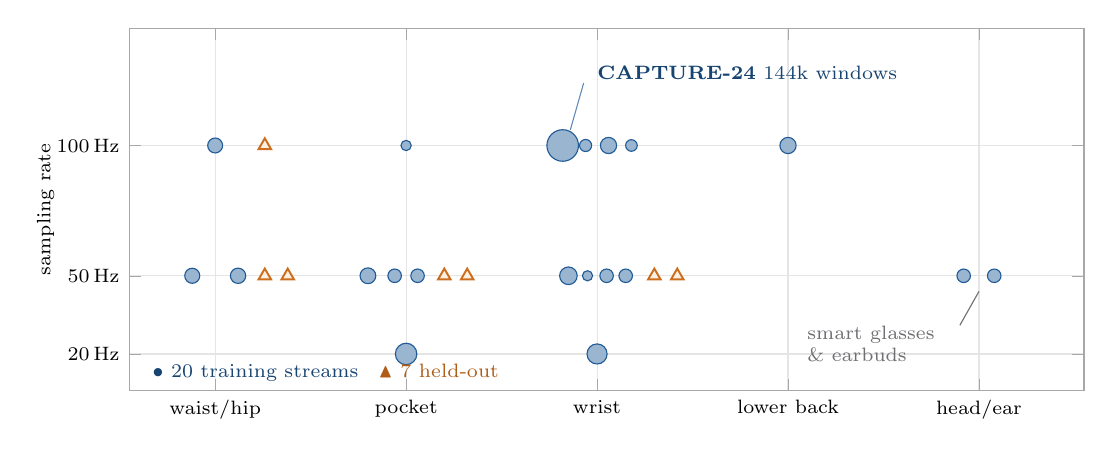
\begin{tikzpicture}
\begin{axis}[
  width=\columnwidth, height=4.6cm,
  xmin=0.55, xmax=5.55,
  ymin=6, ymax=145,
  ytick={20,50,100},
  yticklabels={20\,Hz,50\,Hz,100\,Hz},
  yticklabel style={font=\scriptsize},
  xtick={1,2,3,4,5},
  xticklabels={waist/hip,pocket,wrist,lower back,head/ear},
  xticklabel style={font=\scriptsize},
  ylabel={sampling rate},
  ylabel style={font=\scriptsize,yshift=-6pt},
  grid=major, grid style={draw=halogray!18},
  axis line style={draw=halogray!60},
  tick style={draw=halogray!60},
  scale only axis,
  clip=false,
]
% ---------- training streams (filled blue discs, diameter ~ #windows^0.4) ----
% diameters below are 2*(1.2 + 4.5*(n/144142)^0.4) pt, n = window count
\tikzset{hdisc/.style={circle,draw=haloblue,fill=haloblue!45,line width=0.4pt,inner sep=0pt}}
\node[hdisc,minimum size=5.44pt] at (axis cs:0.88,50)  {};% hhar        9,587
\node[hdisc,minimum size=5.40pt] at (axis cs:1.00,100) {};% kuhar       9,233
\node[hdisc,minimum size=5.54pt] at (axis cs:1.12,50)  {};% uci_har    10,299
\node[hdisc,minimum size=5.70pt] at (axis cs:1.80,50)  {};% unimib     11,771
\node[hdisc,minimum size=4.88pt] at (axis cs:1.94,50)  {};% xrf l.pkt   5,794
\node[hdisc,minimum size=7.76pt] at (axis cs:2.00,20)  {};% wisdm pkt  39,329
\node[hdisc,minimum size=4.88pt] at (axis cs:2.06,50)  {};% xrf r.pkt   5,794
\node[hdisc,minimum size=3.72pt] at (axis cs:2.00,100) {};% spsw pkt    1,179
\node[hdisc,minimum size=11.4pt] at (axis cs:2.82,100) {};% capture24 144,142
\node[hdisc,minimum size=6.36pt] at (axis cs:2.85,50)  {};% harmes     18,576
\node[hdisc,minimum size=4.36pt] at (axis cs:2.94,100) {};% pamap2      3,186
\node[hdisc,minimum size=3.68pt] at (axis cs:2.95,50)  {};% mhealth     1,104
\node[hdisc,minimum size=7.26pt] at (axis cs:3.00,20)  {};% wisdm wr   30,876
\node[hdisc,minimum size=4.88pt] at (axis cs:3.05,50)  {};% xrf l.wr    5,794
\node[hdisc,minimum size=5.86pt] at (axis cs:3.06,100) {};% nfi wrist  13,260
\node[hdisc,minimum size=4.88pt] at (axis cs:3.15,50)  {};% xrf r.wr    5,794
\node[hdisc,minimum size=4.20pt] at (axis cs:3.18,100) {};% spsw wrist  2,578
\node[hdisc,minimum size=5.86pt] at (axis cs:4.00,100) {};% nfi back   13,260
\node[hdisc,minimum size=4.88pt] at (axis cs:4.92,50)  {};% xrf glasses 5,794
\node[hdisc,minimum size=4.88pt] at (axis cs:5.08,50)  {};% xrf earbuds 5,794
% ---------- held-out datasets (open orange triangles) ----------
\addplot[only marks,mark=triangle*,mark size=2.6pt,color=haloorange,
         fill=halolight2,line width=0.7pt]
  coordinates {
    (1.26,50) (1.38,50) (1.26,100)
    (2.20,50) (2.32,50)
    (3.30,50) (3.42,50)
  };
% ---------- annotations ----------
\node[font=\scriptsize,color=haloblue!75!black,anchor=west] at (axis cs:2.95,128)
  {\textbf{CAPTURE-24} 144k windows};
\draw[haloblue!70,thin] (axis cs:2.86,106) -- (axis cs:2.93,124);
\node[font=\scriptsize,color=halogray,anchor=west,align=left] at (axis cs:4.05,24)
  {smart glasses\\ \& earbuds};
\draw[halogray,thin] (axis cs:5.00,44) -- (axis cs:4.90,31);
\node[font=\scriptsize,anchor=west,align=left] at (axis cs:0.62,13)
  {\textcolor{haloblue!75!black}{$\bullet$ 20 training streams}\;\;
   \textcolor{haloorange!85!black}{$\blacktriangle$ 7 held-out}};
\end{axis}
\end{tikzpicture}}
\caption{\textbf{The corpus does not cover a grid; it covers a scatter.} Each blue disc is
one of the 20 sensor streams HALO trains on, positioned by body placement and native
sampling rate, with area proportional to the number of $6$\,s windows it contributes; orange
triangles are the 7 held-out evaluation datasets. Rates span a $5\times$ range and placements
include two---smart glasses and wireless earbuds---that no established HAR benchmark
contains. Held-out cells are not simply new subjects: they combine placements and rates in
proportions the training corpus never sees. Absorbing this by resampling to a common rate
would discard the content above $10$\,Hz that only the $50$/$100$\,Hz streams can
resolve.}
\label{fig:corpus}

\end{figure}

\begin{figure*}[t]
    \centering
    \setlength{\abovecaptionskip}{4pt}
    \setlength{\belowcaptionskip}{-6pt}
  \resizebox{0.92\textwidth}{!}{% Retired from the manuscript. The former teaser embedded trace values without
% a checked-in generator that bound them to source windows and artifact hashes.
% Reintroduce it only with provenance-complete generated data.
}
  \caption{\textbf{What ``no closed grammar'' looks like in the corpus.} The three traces on the
  left are real accelerometer snippets of \emph{walking}, two seconds each, from three streams of
  the materialised corpus; they are amplitude-normalised for display, but the sample counts are
  the true ones. As arrays they have nothing in common. HALO absorbs that heterogeneity
  \emph{in the tokenizer}---a frequency axis fixed in Hz, sensor identity supplied in language,
  gravity preserved---so windows recorded on different devices become directly comparable as
  vectors, which is the precondition for one flat memory. Recognition is then a retrieval in
  \emph{sensor} space, with the label strings a deployment declares at run time used only to name
  and to enumerate; because the memory is append-only, one frozen model spans the whole label
  budget with no gradient update at any point.}
  \label{fig:hook}
\end{figure*}

\textbf{Deliberate exclusions.} Six datasets were excluded from both splits.
DSADS~\cite{dsads}, HARTH~\cite{harth}, and Opportunity~\cite{opportunity} use torso and limb IMU
harnesses rather than phone or watch placements. RecGym~\cite{recgym} is distributed per-axis
min--max normalised, which destroys the physical scale and gravity component the tokenizer
depends on. MobiAct~\cite{mobiact} was never materialised into grids. And HAPT~\cite{hapt} is
excluded because it re-records the same 30 subjects as UCI-HAR~\cite{ucihar}, so including both
would place the same people on both sides of a supposedly subject-disjoint boundary.

\section{Baselines}
\label{app:baselines}

Table~\ref{tab:baselines} lists the five baselines, what each was pretrained on, and how much
acquisition context each can receive at inference---the axis on which the comparison is not
symmetric.

\begin{table}[h]
  \centering
  \caption{Baselines and where each sits on the heterogeneity stack. ``Blind'' means the model
  receives no information about where the sensor was worn. Two baselines are pretrained by us on
  our corpus with their published objectives (data-matched); three are used as released
  (faithful, but pretrained on their own, larger corpora). We report the two groups separately
  rather than averaging over them.}
  \label{tab:baselines}
  \scriptsize
  \setlength{\tabcolsep}{2.5pt}
  \begin{tabular}{@{}l l l l l@{}}
    \toprule
    Model & Weights & Rate & Channels / placement & Labels \\
    \midrule
    LiMU-BERT~\cite{limubert}   & we pretrain & 20\,Hz & 6-ch pad$+$mask; blind & ConSE \\
    CrossHAR~\cite{crosshar}    & we pretrain & 20\,Hz & 6-ch pad$+$mask; blind & ConSE \\
    harnet~\cite{sslwearables}  & released    & 30\,Hz & 3-ch acc; wrist & ConSE \\
    UniMTS~\cite{unimts}        & released    & resamp. & joint-graph placement & native \\
    NormWear~\cite{normwear}    & released    & 65\,Hz & variable ch; blind & native \\
    \midrule
    \textbf{HALO} (ours)        & we train    & \textbf{native} & \textbf{per-sensor language} & \textbf{native} \\
    \bottomrule
  \end{tabular}
\end{table}

\section{Parity Control}
\label{app:parity}

Because several baselines cannot accept HALO's native inputs, Table~\ref{tab:parity} reports HALO
restricted to each baseline's own input contract, so any remaining gap is attributable to the
model rather than to what it was allowed to read.

\begin{table}[h]
  \centering
  \caption{Parity control: HALO under its native inputs versus baseline-equivalent inputs.
  Baselines are split by whether their weights were trained on our corpus or released by their
  authors.}
  \label{tab:parity}
  \scriptsize
  \setlength{\tabcolsep}{6pt}
  \begin{tabular}{l cc}
    \toprule
    Configuration & $k{=}0$ & $k{=}10$ \\
    \midrule
    HALO (native Hz, per-sensor text)          & \PH & \PH \\
    HALO \emph{parity} (20\,Hz, neutral text)  & \PH & \PH \\
    \midrule
    Best baseline (data-matched group)         & \PH & \PH \\
    Best baseline (released-checkpoint group)  & \PH & \PH \\
    \bottomrule
  \end{tabular}
\end{table}

\section{Gravity as a Signed DC Feature}
\label{app:gravity}

Section~\ref{sec:sensor_grouping} keeps the quasi-static component as a signed per-axis feature
rather than normalising it away. Figure~\ref{fig:gravity} is the measurement behind that choice.

\begin{figure*}[t]
    \centering
    \setlength{\abovecaptionskip}{4pt}
  \resizebox{0.86\textwidth}{!}{% Retired on 2026-08-17. The previous posture similarities lacked a checked-in generating script,
% input-window manifest, and raw output. Reintroduce only after the signed-low-frequency ablation is
% reproduced and registered in EVIDENCE_LEDGER.md.
}
  \caption{\textbf{Why gravity is conditioned on rather than normalised away.} Three static
  postures, UCI-HAR waist phone, $200$ windows each through the real tokenizer path.
  \emph{Left:} the frequency path receives almost nothing (note the $\times10^{-3}$ axis) and
  separates no pair distinctly---all pairwise cosines fall within $0.84$--$0.88$. \emph{Right:}
  signed DC places lying nearly orthogonal to standing ($-0.04$), because gravity has
  redistributed across axes. The limit is shown too: standing and sitting stay at $0.99$ in DC,
  the same pair Section~\ref{sec:geometry} finds inseparable in text.}
  \label{fig:gravity}
\end{figure*}

\section{Tokenizer Guardrails}
\label{app:tokenizer}

\begin{figure}[h]
    \centering
    \setlength{\abovecaptionskip}{4pt}
  % =====================================================================
% fig_tokenizer.tex  --  the physical-Hz constant-Q filterbank
%
% DATA PROVENANCE: band centers are the exact values the implementation
% builds, c_k = f_min (f_max/f_min)^{k/(K-1)}, K=32, f_min=0.3, f_max=15 Hz
% (model/tokenizer/filterbank.py); sigma_k = c_k/(2Q) with Q=4.  The Nyquist
% guard lines are FB_NYQUIST_MARGIN * r/2 with margin 0.9.  Observable-band
% counts (26/32 at 20 Hz, 27/32 at 25 Hz, 32/32 at 50 and 100 Hz) were
% enumerated from the same constants on 2026-07-26.
% =====================================================================
\resizebox{\columnwidth}{!}{%
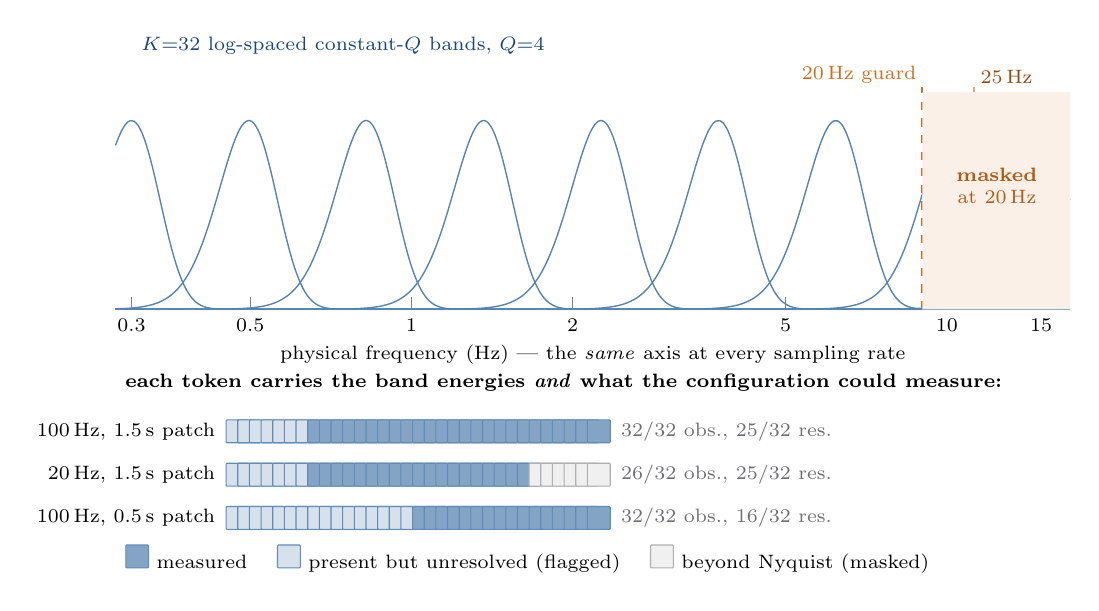
\begin{tikzpicture}[font=\scriptsize]

% ---------------- filterbank response ----------------
\begin{axis}[
  width=\columnwidth, height=3.5cm,
  xmode=log, log basis x=10,
  xmin=0.28, xmax=17, ymin=0, ymax=1.46,
  xtick={0.3,0.5,1,2,5,10,15},
  xticklabels={0.3,0.5,1,2,5,10,15},
  xticklabel style={font=\scriptsize},
  ytick=\empty,
  xlabel={physical frequency (Hz) --- the \emph{same} axis at every sampling rate},
  xlabel style={font=\scriptsize,yshift=2pt},
  axis y line=none, axis x line*=bottom,
  axis line style={draw=halogray!70},
  scale only axis, clip=false,
]
% --- a representative subset of the K=32 log-spaced constant-Q bands (Q=4) ---
\foreach \c in {0.300,0.497,0.823,1.364,2.259,3.743,6.201,10.272,15.000} {
  % the max(-25,.) clamp keeps pgfmath's exp() from underflowing to a
  % "Dimension too large" error in the far tails of the narrow low-Hz bands
  \edef\tmp{\noexpand\addplot[domain=0.28:17,samples=260,smooth,draw=haloblue!75,
      line width=0.5pt]{exp(max(-25,-((x-\c)^2)/(2*(\c/8)^2)))};}
  \tmp
}
% --- Nyquist guard lines ---
\addplot[dashed,line width=0.7pt,draw=haloorange] coordinates {(9.0,0) (9.0,1.18)};
\addplot[dashed,line width=0.7pt,draw=haloorange!60] coordinates {(11.25,0) (11.25,1.18)};
\node[font=\scriptsize,color=haloorange,anchor=south east,inner sep=1pt]
  at (axis cs:8.9,1.18) {20\,Hz guard};
\node[font=\scriptsize,color=haloorange!70!black,anchor=south west,inner sep=1pt]
  at (axis cs:11.4,1.18) {25\,Hz};
% --- masked-band shading ---
\addplot[draw=none,fill=haloorange!10,forget plot]
  coordinates {(9.0,0) (17,0) (17,1.15) (9.0,1.15)} \closedcycle;
\node[font=\scriptsize,color=haloorange!85!black,anchor=north,align=center]
  at (axis cs:12.4,0.80) {\textbf{masked}\\ at 20\,Hz};
\node[font=\scriptsize,color=haloblue!80!black,anchor=south west]
  at (axis cs:0.30,1.30) {$K{=}32$ log-spaced constant-$Q$ bands, $Q{=}4$};
\end{axis}

% ---------------- what the token actually carries ----------------
% Real mask vectors from PhysicalFilterbankTokenizer._observability_masks
% at the three (rate, patch-duration) combinations named on the left.
\begin{scope}[yshift=-1.55cm, xshift=1.55cm]
\node[font=\scriptsize\bfseries,anchor=west] at (-1.55,0.62)
  {each token carries the band energies \emph{and} what the configuration could measure:};
\node[fbblur] at (0.000,-0.000) {};
\node[fbblur] at (0.148,-0.000) {};
\node[fbblur] at (0.296,-0.000) {};
\node[fbblur] at (0.444,-0.000) {};
\node[fbblur] at (0.592,-0.000) {};
\node[fbblur] at (0.740,-0.000) {};
\node[fbblur] at (0.888,-0.000) {};
\node[fbok] at (1.036,-0.000) {};
\node[fbok] at (1.184,-0.000) {};
\node[fbok] at (1.332,-0.000) {};
\node[fbok] at (1.480,-0.000) {};
\node[fbok] at (1.628,-0.000) {};
\node[fbok] at (1.776,-0.000) {};
\node[fbok] at (1.924,-0.000) {};
\node[fbok] at (2.072,-0.000) {};
\node[fbok] at (2.220,-0.000) {};
\node[fbok] at (2.368,-0.000) {};
\node[fbok] at (2.516,-0.000) {};
\node[fbok] at (2.664,-0.000) {};
\node[fbok] at (2.812,-0.000) {};
\node[fbok] at (2.960,-0.000) {};
\node[fbok] at (3.108,-0.000) {};
\node[fbok] at (3.256,-0.000) {};
\node[fbok] at (3.404,-0.000) {};
\node[fbok] at (3.552,-0.000) {};
\node[fbok] at (3.700,-0.000) {};
\node[fbok] at (3.848,-0.000) {};
\node[fbok] at (3.996,-0.000) {};
\node[fbok] at (4.144,-0.000) {};
\node[fbok] at (4.292,-0.000) {};
\node[fbok] at (4.440,-0.000) {};
\node[fbok] at (4.588,-0.000) {};
\node[font=\scriptsize,anchor=east] at (-0.16,-0.000) {100\,Hz, 1.5\,s patch};
\node[font=\scriptsize,anchor=west,color=halogray] at (4.748,-0.000) {32/32 obs., 25/32 res.};
\node[fbblur] at (0.000,-0.550) {};
\node[fbblur] at (0.148,-0.550) {};
\node[fbblur] at (0.296,-0.550) {};
\node[fbblur] at (0.444,-0.550) {};
\node[fbblur] at (0.592,-0.550) {};
\node[fbblur] at (0.740,-0.550) {};
\node[fbblur] at (0.888,-0.550) {};
\node[fbok] at (1.036,-0.550) {};
\node[fbok] at (1.184,-0.550) {};
\node[fbok] at (1.332,-0.550) {};
\node[fbok] at (1.480,-0.550) {};
\node[fbok] at (1.628,-0.550) {};
\node[fbok] at (1.776,-0.550) {};
\node[fbok] at (1.924,-0.550) {};
\node[fbok] at (2.072,-0.550) {};
\node[fbok] at (2.220,-0.550) {};
\node[fbok] at (2.368,-0.550) {};
\node[fbok] at (2.516,-0.550) {};
\node[fbok] at (2.664,-0.550) {};
\node[fbok] at (2.812,-0.550) {};
\node[fbok] at (2.960,-0.550) {};
\node[fbok] at (3.108,-0.550) {};
\node[fbok] at (3.256,-0.550) {};
\node[fbok] at (3.404,-0.550) {};
\node[fbok] at (3.552,-0.550) {};
\node[fbok] at (3.700,-0.550) {};
\node[fbno] at (3.848,-0.550) {};
\node[fbno] at (3.996,-0.550) {};
\node[fbno] at (4.144,-0.550) {};
\node[fbno] at (4.292,-0.550) {};
\node[fbno] at (4.440,-0.550) {};
\node[fbno] at (4.588,-0.550) {};
\node[font=\scriptsize,anchor=east] at (-0.16,-0.550) {20\,Hz, 1.5\,s patch};
\node[font=\scriptsize,anchor=west,color=halogray] at (4.748,-0.550) {26/32 obs., 25/32 res.};
\node[fbblur] at (0.000,-1.100) {};
\node[fbblur] at (0.148,-1.100) {};
\node[fbblur] at (0.296,-1.100) {};
\node[fbblur] at (0.444,-1.100) {};
\node[fbblur] at (0.592,-1.100) {};
\node[fbblur] at (0.740,-1.100) {};
\node[fbblur] at (0.888,-1.100) {};
\node[fbblur] at (1.036,-1.100) {};
\node[fbblur] at (1.184,-1.100) {};
\node[fbblur] at (1.332,-1.100) {};
\node[fbblur] at (1.480,-1.100) {};
\node[fbblur] at (1.628,-1.100) {};
\node[fbblur] at (1.776,-1.100) {};
\node[fbblur] at (1.924,-1.100) {};
\node[fbblur] at (2.072,-1.100) {};
\node[fbblur] at (2.220,-1.100) {};
\node[fbok] at (2.368,-1.100) {};
\node[fbok] at (2.516,-1.100) {};
\node[fbok] at (2.664,-1.100) {};
\node[fbok] at (2.812,-1.100) {};
\node[fbok] at (2.960,-1.100) {};
\node[fbok] at (3.108,-1.100) {};
\node[fbok] at (3.256,-1.100) {};
\node[fbok] at (3.404,-1.100) {};
\node[fbok] at (3.552,-1.100) {};
\node[fbok] at (3.700,-1.100) {};
\node[fbok] at (3.848,-1.100) {};
\node[fbok] at (3.996,-1.100) {};
\node[fbok] at (4.144,-1.100) {};
\node[fbok] at (4.292,-1.100) {};
\node[fbok] at (4.440,-1.100) {};
\node[fbok] at (4.588,-1.100) {};
\node[font=\scriptsize,anchor=east] at (-0.16,-1.100) {100\,Hz, 0.5\,s patch};
\node[font=\scriptsize,anchor=west,color=halogray] at (4.748,-1.100) {32/32 obs., 16/32 res.};
\node[font=\scriptsize,anchor=west,align=left] at (-1.55,-1.62)
  {\tikz\node[fbok]{};\ measured \quad
   \tikz\node[fbblur]{};\ present but unresolved (flagged) \quad
   \tikz\node[fbno]{};\ beyond Nyquist (masked)};
\end{scope}
\end{tikzpicture}}


  \caption{\textbf{The filterbank, and what a token carries.} \emph{Top:} $K{=}32$ Gaussian bands
  log-spaced over $0.3$--$15$\,Hz; because a native-rate zero-padded rDFT maps bin $m$ to $mr/S$,
  one bank reads every rate without resampling. Dashed lines mark the Nyquist guard for the two
  lowest corpus rates. \emph{Bottom:} the real observability and resolution vectors emitted
  alongside the energies---part of the token, not diagnostics.}
  \label{fig:tokenizer}
\end{figure}

Zero-padding beyond the true patch length is frequency-domain interpolation only and does not
alter band energies; we verified that $S{=}256$ and $S{=}512$ give band-energy cosine $1.000000$
and identical masks at $20$, $25$, $50$, and $100$\,Hz. Patch lengths exceeding $S$ raise an error
rather than silently truncating.

\section{Phase-A Specification}
\label{app:phasea}

The EMA teacher is updated only after an optimizer step (decay $0.996$) and is checkpointed with
the model. Cross-placement positives are drawn under a quota so that the six-placement recordings
cannot dominate; positive identity comes from explicit physical-event identifiers written during
conversion and carried into the pretraining index, never inferred from equal array lengths or row
alignment, and never from an activity label. Per-objective gradient norms, VICReg component
values, minimum feature standard deviation, effective rank, and positive similarity by pair type
are logged every step; non-finite values or representation collapse fail the run rather than
being smoothed over.

\section{Phase-A Objective Ablation}
\label{app:objectives}

\begin{table}[h]
  \centering
  \caption{Phase-A objective ablation, macro-F1 over the held-out datasets. The last two rows are
  controls, not variants: they test whether the non-contrastive and label-free choices were worth
  making.}
  \label{tab:objective_ablation}
  \scriptsize
  \setlength{\tabcolsep}{3pt}
  \begin{tabular}{l cc}
    \toprule
    Phase-A configuration & $k{=}0$ & $k{=}10$ \\
    \midrule
    Full (A1 fixed$+$EMA, VICReg, TF, placement, rail) & \PH & \PH \\
    \quad$-$ EMA-latent target (fixed A1 only)      & \PH & \PH \\
    \quad$-$ augmentation VICReg                    & \PH & \PH \\
    \quad$-$ time--frequency consistency            & \PH & \PH \\
    \quad$-$ cross-placement positives              & \PH & \PH \\
    \quad$-$ physical grounding rail                & \PH & \PH \\
    \midrule
    VICReg $\rightarrow$ NT-Xent (contrastive control) & \PH & \PH \\
    Label-supervised recipe (SupCon; \emph{uses labels}) & \PH & \PH \\
    \bottomrule
  \end{tabular}
\end{table}

\section{Phase-B Episodic Training}
\label{app:phaseb}

The decoder is trained on episodes that vary, independently: the candidate budget
($10$--$100\%$ of the vocabulary); the number of true-label memory exemplars
($0$, $1$, $2$, $4$, $8$, or all); the support available for competing labels; whether memory is
same-configuration, cross-configuration only, or missing the query's configuration entirely; the
kind of distractors present (random, language-near, motion-family-near, physically confusable);
and whether the truth is present at all. Complete label \emph{families} are held out of decoder
training and reserved for model selection, so candidate-text reasoning is always tested on
concepts the decoder never fit. Head collapse in the retrieval projections is resisted by output
decorrelation, projection diversity, and contribution-usage regularisation.


\end{document}